% PLEASE FILL IN THE PLACEHOLDERS <...>
%
% Diplomarbeit/Studienarbeit/IDP von <NAME>
% Diploma thesis of <NAME>
%
% Title: <TITLE>
%        <TITLE>
%
\documentclass[12pt, a4paper, twoside, openright]{report}

%%%%%%%%%%%%%%%%%%%%%%%%%%%%%%%%%%%%%%%%%%%%%%%%%%%%%%%%%%%%

% PACKAGES:

% Define typearea
% a) Use automatic:
\usepackage[BCOR1cm]{typearea}
% b) Or use fixed: 
%\usepackage{geometry}
%\geometry{left=1.5cm,textwidth=18.5cm,top=1.5cm,textheight=26.5cm}

% Use German :
\usepackage[german, english]{babel}
% Use list of tabels, etc. in table of contents:
\usepackage{tocbibind}
% German paragraph skip
\usepackage{parskip}
% Encoder:????
%\usepackage[utf-8]{inputenc}
\usepackage[utf8]{inputenc}
% Use A4-paper efficiently:
\usepackage{a4wide}
% Index-generation
\usepackage{makeidx}
% Einbinden von URLs:
\usepackage{url}
% Include .eps-files (needed also for the LKN-logo):
%\usepackage{epsf}
\usepackage{epsfig}
\usepackage{epstopdf}
% Special \LaTex symbols (e.g. \BibTeX):
\usepackage{doc}
% Include Graphic-files:
%\usepackage{graphics}
% Include Graphic-files:
\usepackage{graphicx}
% Include doc++ generated tex-files:
%\usepackage{docxx}
% Include PDF links
%\usepackage[pdftex, bookmarks=true]{hyperref}
\usepackage{float}
\usepackage{tabularx}
\usepackage[margin=1cm,font=small,labelfont=bf,textfont=sl]{caption}
\usepackage{mathtools}
\usepackage{natbib}

\usepackage[pdftex,
  bookmarks,
  %colorlinks=false, % instead of colors, now boxes are used for links
  colorlinks=true,
  urlcolor=black, %blue,
  linkcolor=black, %red, %normal internal links
  citecolor=black, %green, %citation links
  %pagebackref, %link from references back to page of citation
  linktocpage, 
  % im Inhaltsverzeichnis Link auf Seitenzahl (sonst Probleme bei langen Zeilen)
  %breaklinks = true, % f�r Links l�nger als 1 Zeile
  %hypertexnames = false,  % f�r Links zu Figures?
  bookmarksopen, %open all bookmark folders
  bookmarksnumbered, %use section numbers with bookmarks
    pdfpagemode=UseOutlines, %show bookmarks
  % http://www.tex.ac.uk/cgi-bin/texfaq2html?label=pdfpagelabels
  plainpages=false, % eigene Seitenanker f�r r�mische/arabische Seitenzahlen
  pdfpagelabels, % im Abode Reader Seitenzahl als z.B. "iii (3 von 20)" anzeigen
% pdfstartview=FitH
  pdfstartview=FitV
  ]{hyperref}

%%%%%%%%%%%%%%%%%%%%%%%%%%%%%%%%%%%%%%%%%%%%%%%%%%%%%%%%%%%%

% SELF DEFINED:
%
% this makes list spacing much better.
%
\newenvironment{my_enumerate}{
\begin{enumerate}
  \setlength{\itemsep}{1pt}}{\end{enumerate}
}
\DeclareMathOperator*{\argmax}{arg\,max}
\newcommand{\sml}[1]{\mbox{\scriptsize $#1$}}

%%%%%%%%%%%%%%%%%%%%%%%%%%%%%%%%%%%%%%%%%%%%%%%%%%%%%%%%%%%%

% OTHER SETTINGS:

% Pagestyle:
\pagestyle{headings}

% Avoid 'overhang':
\sloppy

% Choose language
\newcommand{\setlang}[1]{\selectlanguage{#1}\nonfrenchspacing}

%%%%%%%%%%%%%%%%%%%%%%%%%%%%%%%%%%%%%%%%%%%%%%%%%%%%%%%%%%%%

% TITLE:

\begin{document}

\thispagestyle{empty}
\newpage

\vspace{5cm}
\begin{center}
    \epsfxsize=4cm
    \epsfbox{LKN_Logo_klein.eps}
\end{center}

\parbox{15cm}{\begin{center} {\sf\bf 
                               \Large  Technische Universität München
                                \smallskip

                               \Large Lehrstuhl für Kommunikationsnetze
                               \smallskip
                              }

                              {\sf \large Prof. Dr.-Ing. Wolfgang Kellerer} 
              \end{center}}  %&

\vspace{4cm}

\begin{center}
        {\bf\Huge Master‘s Thesis} % Studienarbeit, Interdisziplinäres Projekt
\end{center}

\begin{center}
        \settowidth{\baselineskip}{0.4cm}
        {\LARGE 
        Title of the Thesis
        }
\end{center}

\vfill         
{\settowidth{\baselineskip}{0.2cm}
\large\begin{tabular}[l]{ll}
Author: & Last Name, First Name\\
Address: & Somestreet 007\\
         & 12345 City\\
         & Country\\
Matriculation Number: & XXXXXXX\\
Supervisor: & Supervisor Name\\
Begin: & 01. January 1900\\
End: & 01. January 2000
\end{tabular}}

%%%%%%%%%%%%%%%%%%%%%%%%%%%%%%%%%%%%%%%%%%%%%%%%%%%%%%%%%%%%
\pagenumbering{roman}

\newcounter{pageno}
\setcounter{pageno}{1} %titlepage = page 1, but pagenumber not printed
\addtocounter{pageno}{1}

% German abstract:
%\include{Kurzfassung}
% English abstract:
\pdfbookmark[1]{Abstract}{sec:abstract}  % Bookmark im pdf file
\chapter*{Abstract}
\label{sec:abstract}
A short abstract of the thesis in English. 





\cleardoublepage
\pdfbookmark[1]{Statement}{sec:statement}  % Bookmark im pdf file
\chapter*{Statement}
\label{sec:statement}

\vspace{3cm}
\noindent I assure the single handed composition of this master's thesis only supported by declared resources.\\\\
%M�nchen, DD.MM.YYYY \\\\\\\\\\\\


\vspace*{\fill}

Hamburg, 19. December 2016

\noindent \textit{(John Doe)}

\cleardoublepage
%!TEX root = ThesisLKN.tex
\pdfbookmark[1]{Foreword}{sec:vorwort}  % Bookmark im pdf file
\chapter*{Foreword}
\label{sec:vorwort}

I would like to use this opportunity to express my gratitude to my supervisor Johannes D\"ollinger and his colleague Markus Spies in Bosch, who inspired me a lot during this thesis work. I am also appreciated for the help and guidance I received from Prof. Alexander Schl\"afer and Prof. Dr.-Ing. habil. Udo Z\"olzer. 

Special thanks to all my friends who make my life more enjoyable. Lastly, I sincerely thank my families. Their continuous supports and cares encourage me to step forward. With their love, I know I would never stop. \\




% Table of contents:
\tableofcontents  
%%$$$$$$$$$$$$$$$ tableofcontents $$$$$$$$$$$$$$$$$

\newcommand{\chapname}{Chapter}

\setlength{\parskip}{0ex}
\renewcommand{\baselinestretch}{1}
\normalsize

\cleardoublepage % to get correct page no. in TOC
\pdfbookmark[1]{\contentsname}{toc}  % Bookmark auf Inhaltsverzeichnis im pdf file
%\tableofcontents


\setlength{\parskip}{1ex}
\cleardoublepage % to get correct page no. in TOC
\phantomsection
%\setcounter{lofdepth}{2}
% subfigures werden mit aufgelistet in der LOF
\addcontentsline{toc}{chapter}{\protect\numberline{\listfigurename}}
\listoffigures

\cleardoublepage % to get correct page no. in TOC
\phantomsection
\addcontentsline{toc}{chapter}{\protect\numberline{\listtablename}}
\listoftables

% \cleardoublepage % to get correct page no. in TOC
% \phantomsection
% \addcontentsline{toc}{chapter}{\protect\numberline{\lstlistlistingname}}
% \lstlistoflistings


\renewcommand{\baselinestretch}{1.0}
\normalsize

\cleardoublepage % to get correct page no. in TOC

%\setlength{\parskip}{\parspacing}

\clearpage
\renewcommand{\chaptername}{\chapname} %if name appears in header

% % Introduction (Einleitung):
% \include{Introduction}

% % Text Body (Hauptteil)
% % Could have multiple chaper-files, e.g.:
% \chapter{Background}

\section{Content}
In this chapter, all background necessary to understand the thesis are introduced. The level of detail is such that a colleague with similar background (no specialist!) is capable of understanding the contribution and impact of the thesis. A discussion of state-of-the-art solutions (e.g. literature research) is often helpful. Problems of the state-of-the-art are typically discussed and the contribution of the thesis is introduced in detail. 

% \include{Evaluation}
% %  Conclusions (Zusammenfassung):
% \include{Conclusions}
% \chapter{Formatting}

\section{Figures and Tables}
Figures and tables need to include a caption. This can be done with the LaTeX-command \texttt{\bslash caption$\lbrace\rbrace$}. To be able to reference figures and tables, a \texttt{\bslash label$\lbrace\rbrace$} must follow the caption.

\begin{figure}[h!]
  \begin{center}
    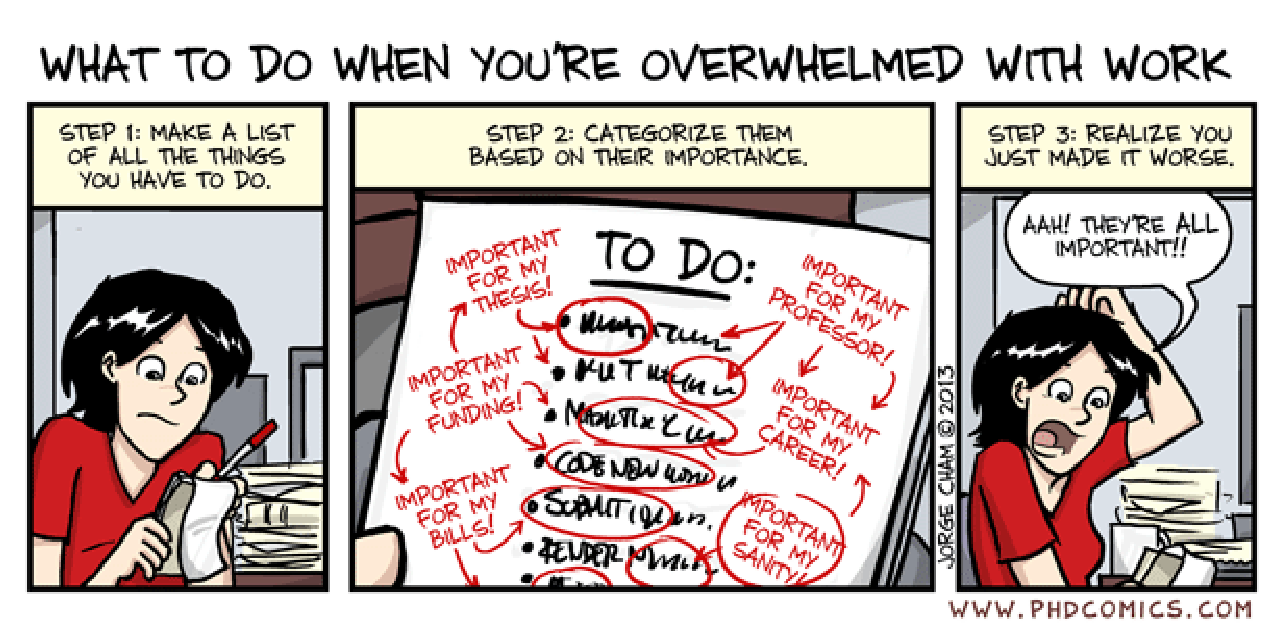
\includegraphics[width=0.6\textwidth]{phd112013s.eps}
    \caption{Ein PHD Comic}
    \label{fig:ToUseWithReference}
  \end{center}
\end{figure}

\begin{table}[b]
\begin{center}
\begin{tabular}{|l |c|}
\hline 
\textbf{Parameter} & \textbf{Value} \\
\hline  
\hline 
Transmission Power & 23~dBm\\
\hline 
Center Frequency & 2.6~GHz\\
\hline 
Channel Bandwidth & 15~kHz\\
\hline 
Shadowing Correlation Distance & 40~m\\
\hline 
Noise Density & -174~dBm/Hz\\
\hline 
Antenna Heights & 1.5~m\\
\hline 
\end{tabular}
\caption{Simulation Parameters and Values}\label{tab:param_table}
\end{center}
\end{table}

The labelled figures and tables can be referenced via \texttt{\bslash ref}, e.g. ~Figure~\ref{fig:ToUseWithReference}.
\newpage


\cleardoublepage
\setcounter{page}{1}
\renewcommand{\thepage}{\arabic{page}}

%!TEX root = ThesisLKN.tex
\chapter{Introduction}

In recent years, more and more robots are deployed in not only industrial environments but also human populated areas. In order to fulfill their tasks, it is necessary for robots to interact and even cooperate with people. Therefore, tracking the locations of people in those environments has gained enormous attentions in robotics community. Besides, with the increasing popularity of artificial intelligence, robots are also expected to be intelligent enough to predict possible future locations of walking human even when encountered with occlusions or missing of sensor data. Enabled with an accurate tracking and prediction of human movements, robots are able to have a better understanding of the environment, which will facilitate interactions between robots and human.

The very fist requirement for a robot to operate is to model the environment. A simple yet effective way is to use occupancy grid map representation of the environment \citep{elfes1989using}. It decomposes the environment into cells with a predefined resolution, and the state of each cell is a random variable with values of either \textit{occupied} or \textit{not occupied}. This representation has been extensively used in many different kind of robot tasks like simultaneous localization and mapping (SLAM). The classical grid map representation treats the environment as static, which is not always the case in real scenarios. In other words, the environment can be dynamic since objects can move around in the environment. Object tracking addresses dynamics in environment explicitly, since it tracks and predicts how objects move. If there are more than one object involved at the same time, the tracking problem becomes multiple object tracking (MOT). In people tracking systems, the dynamics in environment refer to people location changes along the time horizon (i.e., trajectories). 

Commonly, a tracking system is implemented as a multiple stage pipeline, which consists of object detection, data association, motion modeling and occupancy generation. When deal with a multiple object tracking problem, data association becomes very tricky. The classical way to perform data association is to maintain a list of known objects, and associates new observations with those objects. The main difficulty of this approach is to deal with \textit{birth} (whether observation is from a new object) and \textit{death} (whether a maintained object should be deleted) of tracks explicitly \citep{gauvrit1997formulation}. 

To address the data association problem, \citet{coue2006bayesian} proposed \textit{Bayesian occupancy filter} (BOF), which is an object tracking algorithm based on grid map representation of environment. It essentially avoids data association step in the tracking pipeline, since concepts of \textit{objects} and \textit{tracks} dose not exist in BOF framework. Rather than treat tracking problem from an \textit{object} point of view, BOF addresses tracking from a \textit{cell} perspective. That is to say, tracks are replaced by transitions of occupancies between cells over time. Meanwhile, BOF is robust to object occlusion thanks to the combination of \textit{prediction} and \textit{estimation} steps. This two-step mechanism is well suited for handling the consistency between occupancy predictions and new observations, therefore uncertainties incurred by occlusion is naturally handled in a probabilistic way. Over the past few years, there has been some extensions over BOF proposed in literature \citep{gindele2009bayesian, brechtel2010recursive, llamazares2013dynamic}. 

\begin{figure}[H]
  \centering
    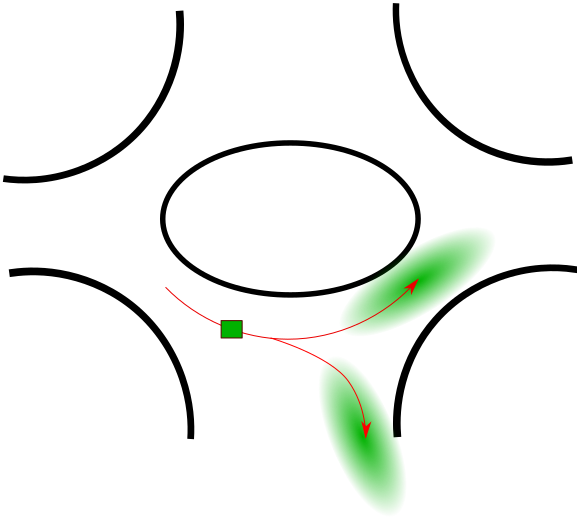
\includegraphics[width=.5\textwidth]{figures/roundabout.png}
    \caption[An illustration of a round-about]{This shows an illustration of a round-about. Cars can only drive in directions indicated by red arrows. The green rectangle represents a car at that location. Since we know that the car must drive in the specified directions, the possible locations of the car after a few time steps are indicated by the two green eclipses. This prior knowledge helps us track the dynamic objects since we have better chances to locate the car according to the motion pattern.}
    \label{fig:roundabout_idea}
\end{figure}

A tracking system usually predicts the state of the world (e.g., object location and velocity) based on past observations. Many tracking algorithms also incorporate motion models of the objects being tracked, since this allows us to utilize prior knowledge of object's motion cues. As an intuitive example, let us consider a round-about as shown in Figure \ref{fig:roundabout_idea}, where cars can only drive in one direction. To track a car driving in a round-about, prediction of next possible locations of the car should always be on the side which allowed driving direction indicates, since we know that the car must follow that direction. Likewise, human tracking in indoor environments can also benefit from human motion patterns. For BOF and its variants, the objects being tracked are assumed to perform linear motion, which indicates that objects always move in the same direction as in the last time step. Although \citet{gindele2009bayesian} proposed to incorporate prior map knowledge (BOFUM) to better model the motion dynamics based on cell context, linear motion is too simplistic to model actual human motion in indoor environments. 

Based on our observations of human trajectories, we found two aspects very important for explaining human motion: 1) Unlike in free space, people have to move under spatial constraints in indoor environments. For example, people tend to walk along the central area between walls in a corridor and change their walking directions when they have to make turns. That is to say, the spatial constraints limit human motion patterns and therefore human motion is very place dependent. 2) People move continuously in time and space, which means they does not disappear or appear out of thin air. If a person is currently at a cell of a grid map, he or she has to walk through its neighboring cells first. In other words, future movement events starting from a region of interests are highly influenced by state changes of its neighboring cells. These observations motivates us to model human motion in a way that captures both \textbf{place dependency} as well as \textbf{spatial correlation} between cells.

In computer vision community, researches in machine learning over last few years has shown a lot of successes. Image classification algorithms based on convolutional neural networks (CNNs) has won all ImageNet classification challenges since 2012 \citep{russakovsky2015imagenet}. It turns out that CNNs can achieve good results in not only computer vision tasks but also many other domains. For example, recurrent neural networks (RNNs) can be applied in automatic language translation \citep{cho2014learning}. Deep reinforcement learning are good choice for teaching robots to perform human actions like grasping\citep{levine2016learning}. Essentially, the reason why CNN works in those domains is that it is able to capture complex structure in data. Once a CNN learns that structure, it can generalize to cases that never occurs during training. 

In order to utilize the powerful generalization abilities of CNNs, we proposed to model motion patterns in a way that can be easily expressed as the output of a CNN. In this way, if we feed a gird map as input and human motion patterns as ground truth to a network, it should be able to learn the patterns after training with lots of data. We model human motion patterns as a set of conditional probabilities for every cell on the map. They represent how likely a person moves to one of the neighboring cells, conditioned on which neighboring cell he or she comes from. Since these probabilities incorporate information about the incoming cell, the motion model captures spatial correlations between cells. Besides, they are different for each cell based on cell's context on the map, which means the learned motion pattern is expressive enough to predict different motions at different locations. In other words, our motion model is place dependent. In fact, similar idea of making motion patterns place dependent has been proposed by \cite{kucner2013conditional}, but in order to learn motion pattern on a map, they need sensor observations from that specific map. In other words, their method lacks of generalization ability. On the contrary, with a large training set, we exploit the power of CNNs so that our method can generalize to maps that have never occurs.

\begin{figure}[H]
  \centering
    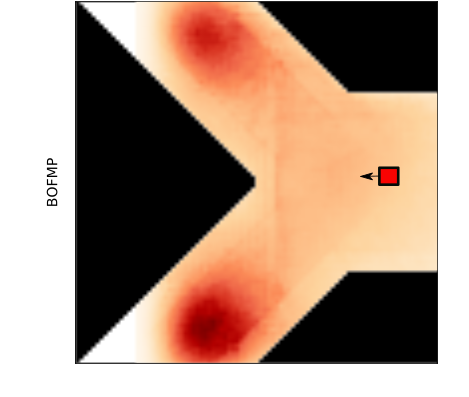
\includegraphics[width=.6\textwidth]{figures/theme_plot_1.png}
    \caption[An example of future occupancy predictions of our method.]{An example of future occupancy predictions of our method.  The map shows a Y-fork, where only white spaces are walkable. Initially, a person is shown as a red rectangle and with velocity towards left. Since no further sensor reading is given, BOFMP propagates occupancies over time. After some time interval, most occupancies appear in both upper and lower branches of the corridor, which proves that our motion model successfully learns that people tend to make turns at the intersection. Besides, our BOFMP predicts more occupancies in the middle of corridors, since it learns that people are less likely to walk near walls.}
    \label{fig:idea}
\end{figure}

The data we use for training network is generated from simulated human walking trajectories on SLAM-generated maps of real world offices. Once the network finishes learning, we can feed new maps to the network and obtain human motion patterns from network outputs. These motion patterns are then incorporated into BOF framework to perform human tracking in indoor environments. We call our tracking method as \textit{Bayesian Occupancy Filter with Motion Patterns} (BOFMP). If only initial state of a person is given and no further observations are provided, our method is able to predict reachable areas after some time steps. Figure \ref{fig:idea} shows an example of future occupancy predictions of our method without sensor observations. It shows that our way of modeling human motion patterns enables BOF to propagate occupancies to reasonable areas.

The main contributions of this thesis work are:

\begin{my_enumerate}
\item We present a way of modeling human motion patterns that captures both place dependency and spatial correlations between cells. Besides, thanks to powerful generalization abilities of CNNs, our method can generate motion patterns on maps that are never seen by our model.
\item We incorporate the learned motion patterns into BOF framework seamlessly for human tracking in indoor environment, and achieve better tracking performance than baseline method.  The whole pipeline of modeling motion pattern and tracking presented in this thesis work can be applied in other scenarios, such as car tracking in ADAS systems.
\end{my_enumerate}


The rest of this thesis is organized as follows: Chapter \ref{chapter:2} summarizes the related works and highlights the similarities and differences between our method and others in literatures. Chapter \ref{chapter:3} introduces how BOF is derived and mathematical formulation of CNNs. Chapter \ref{chapter:4} explains the detailed implementations, such as generation of dataset and BOF. Chapter \ref{chapter:5} summarizes the dataset and presents the tracking performance of our method and the baseline. Chapter \ref{chapter:6} concludes the thesis work and presents possible improvements on our method. 


\cleardoublepage
%!TEX root = ThesisLKN.tex
\chapter{Literature Review} \label{chapter:2}

This chapter lists literatures that are related to methods or concepts used in this thesis work. Section \ref{lr:tracking} discusses two classical ways of tracking object and introduces BOF and its variants. Section \ref{lr:dynamic} presents literatures that try to model dynamics in environment. Section \ref{lr:network} details recent researches on neural networks and relations between RNNs and Bayesian filters. 

\section{Object Tracking} \label{lr:tracking}

Perception of environment can be done with different sensors, which also differentiates object tracking applications. Visual tracking refers to object tracking with RGB cameras \citep{ross2008incremental}. In this thesis work, however, we mainly concern object tracking with 2D laser scanners. 

One popular paradigm of performing tracking is tracking by detection: moving objects are firstly detected and then determine how to pair them with existing tracks. Generally, there are two approaches to deal with detection based object tracking: \textit{model-free} and \textit{model-based} \citep{wang2015model}. The detection of model-free object tracking works based on motion cues. In this case, prior knowledge on neither object's semantic information (whether it is a car or a person) nor object's shape or geometric properties is needed. However, this approach only tracks objects that show instantaneous motion dynamics and potential moving objects might be neglected. BOF can be regraded as a model-free tracking algorithm (but not within tracking by detection paradigm) since it predicts occupancies based on its inference on cells' velocities. Similar to BOF, \citet{ross2008incremental} models the environment with occupancy gird map. Their work combines SLAM with dynamic object tracking in outdoor environment. Once the vehicle equipped with laser sensors is self-located and objects are detected by motion cues, they apply a method called Global Nearest Neighborhood (GNN) for tracking. On the contrary, for model-based tracking, semantic class of the objects being tracked is given, and detection is done with the help of a parametric model of the object's shape. For human tracking, a person is normally represented as point blob or modeled based on detection of legs \citep{arras2008efficient, cui2006laser}. 

The tracking by detection paradigm has to address \textit{data association} explicitly, which is known to be as the main difficulty in tracking. Data associations refers to match detections of moving objects in new observations to a set of tracked trajectories from last time step. To address data association problems in tracking, many methods have been proposed in literature. Historically, nearest neighbors based approaches are used in the early stage \citep{fod2002laser}. \citet{schulz2001tracking} detect people by their legs in 2D laser scans and propose the Joint Probabilistic Data Association Filter (JPDAF) for tracking. \citet{arras2008efficient} is similar in identifying people with legs but their tracking is done with Multi-hypothesis tracking (MHT). Although the mentioned methods partially address the data association problem, their performance is not stable in densely cluttered environments, where occlusions happen quite often.

On the contrary to tracking by detection paradigm, tracking can also be done without detection, e.g., tracking by filtering. \citet{coue2006bayesian} propose Bayesian Occupancy Filter for object tracking in automotive applications. The environment is represented by a grid map, and the state of each cell is characterized by its occupancy and velocity. Inspired by Bayesian Filter, tracking works in a form of recursive \textit{predictions} and \textit{estimations} of cells' state. One of important advantages of BOF is that the concepts of \textit{objects} and \textit{tracks} are replaced by transitions of occupancies between cells over time. That is to say, data association is addressed implicitly by BOF. Later works extend BOF to better adapt to real world situations. BOF's linear motion model cannot adapt to traffic scenarios like curved roads. Therefore, \citet{gindele2009bayesian} propose to enrich motion model of BOF with prior map knowledge (BOFUM), which can be obtained from navigation systems. By this way, BOFUM predicts occupancies according to motion preferences at different locations, which results in reliable estimates even when occlusion happens. 

Despite of various variants of BOF, all of them assume that objects perform linear motion. However, linear motion is obviously over-simplified for real world scenarios. Besides, since objects cannot appear or disappear suddenly, the state changes of a cell's neighboring cells contain valuable information for prediction of its future state. Therefore, we proposed to model human motion patterns in a way that captures both place dependency and spatial correlation of cells. This motion model is then incorporated into BOF framework to perform human tracking. A similar idea is used in the work of \citet{luber2011place}, which proposed a place dependent people tracking algorithm. Unlike BOF which tracks objects by filtering, they perform people tracking by detection and data association. They proposed to model human activity events as a three-layer spatial affordance map with each layer characterizing the probability distribution of new tracks, matched tracks and false alarms respectively. Each layer is represented by a \textit{spatial} Poisson process which introduces spatial dependency and the parameter of each cell is learned from a sequence of observations. Figure \ref{fig:affordance} shows one example of two layers of the learned spatial affordance map. Their motion model is place dependent because the parameters of Poisson processes are different on the spatial affordance map. They use boosted features for people detection \citep{arras2007using} and they extend multiple hypothesis tracking (MHT) for data association. Their results show they achieve more accurate tracking behavior in terms of data association errors. 

\begin{figure}[H]
  \centering
    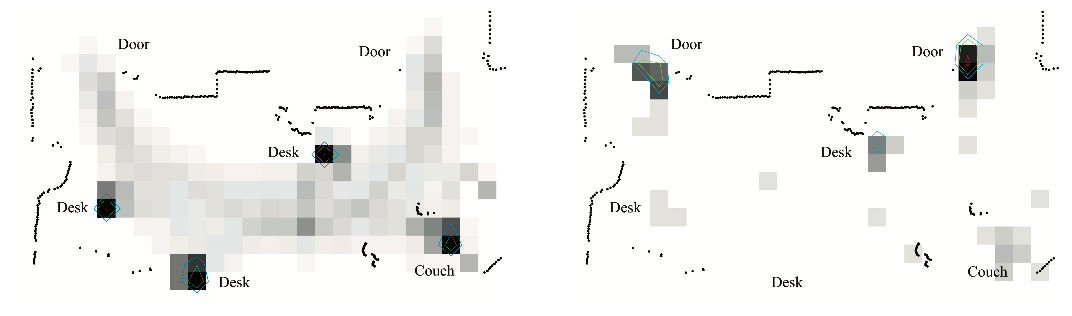
\includegraphics[width=\textwidth]{figures/affordance_map.png}
    \caption[Two layers of a spatial affordance map.]{Two layers of a learned spatial affordance map \citep{luber2011place}. On the left shows probability distribution of matched track events, and on the right shows that of new track events. Note that the maxima appear in different regions in two maps. While on the left the maxima appear at places frequently used by people (e.g., desks and coach), on the right the maxima of new track events indicate places where people normally appear from, i.e., doors.}
    \label{fig:affordance}
\end{figure}

\section{Dynamics Modeling} \label{lr:dynamic}

Nowadays, more and more robots are entering dynamic environments. In order to fulfill their task, it is imperative for robots to understand these dynamics. In the context of human tracking, these dynamics refer to human movements in the environment. In literature, some researchers try to model human dynamics \textit{explicitly} by a motion model. Meanwhile, others model them \textit{implicitly} by regarding human dynamics as part of the environment and therefore model the environment directly. We discuss dynamics modeling according to these two approaches. In both cases, we represent the environment as a gird map with each cell representing a possible location. 

\subsection{Human Motion Modeling}

In the early stage of human tracking, researches adopts simple and conservative motion models. \citet{montemerlo2002conditional} uses Brownian motion model for human tracking with Bayesian filters.  The Brownian motion assumes people take random directions at each time step and there is no dependence between time steps. In other words, Brownian motion does not assign human dynamics with any pattern other than dispersion. As a consequence, when there is no observations, predictions of people locations spread out over a large area very quickly. This is a poor estimate as we know people does not move randomly. In reality, people normally go from the starting point and follow some motion patterns until they reach destination. A more realistic model is the first order motion model (a.k.a. linear motion model). For example, \citet{meier1999using} used this model together with Kalman filter for human tracking. First order motion model assumes people always move in the same direction as in the last time step. This assumption might be true if a person is walking along a straight corridor, but in many cases it is invalid because people often need to make turns around corners. Some researchers proposed better ways to model human motion patterns. For example, \citet{bruce2004better} propose to learn destinations by clustering real trajectories and use a path planer to those destinations as a reference for human motion patterns. \citet{liao2003voronoi} observe that human tend to move along Voronoi graph of the environment and therefore constraint motion patterns by Voronoi graph. 

Our motion model is different to above methods in two aspects: fineness and cell dependency. The Voronoi graph is constructed based on a \textit{global} representation of the environment. It is predefined and only well suited for applications where high-level motion clue is needed (e.g., which rooms a person has visited). This kind of motion clues are too less precise to be used for recovering a person's exact location. Therefore, in order to get a finer motion model, we decompose the \textit{global} task of modeling human motion pattern into \textit{local} tasks at cell level. On the other hand, although a path planer to the learned destination defines an effective path, it does not necessarily cover the motion dynamics at every possible locations and it also assumes no dependency between these locations. One intuition we captured based on observations of human motion is that, for a cell in the map, the state changes of its neighboring cells is a strong indicator for predictions of its future state. To capture this \textit{spatial} correlation, we propose to model changes of movement directions. For each cell, we learn from human trajectories how likely a person's moving direction changes for the next time step, conditioned on the direction with which he or she enters this cell. Moreover, this way of motion modeling also captures \textit{temporal} correlations, since it builds connections for each cell with its neighboring cells from both last time step and next time step. 

In fact, after we came up with above way of modeling human motion, we found in literature the same idea has been used by \citet{kucner2013conditional} in an autonomous navigation scenario. Their model, which is named as Conditional Transition Map, is created by ``learning the probability distribution of an object leaving to a certain neighboring cell, given the cell from which it entered into the current cell.'' They demonstrate their method with a roundabout, and the corresponding model is illustrated in Figure \ref{fig:condi_tran_map}. One can see that at different locations in the roundabout, different motions are learned, which accurately models how cars drive through the roundabout. The difference between our method and theirs lies in how those probabilities are learned. The cross-correlation of temporal occupancy signals extracted from observations is used for learning in their method, while our model learns these probabilities by training a neural network. With lots of different maps as training data, our network is able to learn the motion patterns that are constrained by spatial configurations of these maps. One of the most important advantages of our method is that our network can generalize motion patterns for maps that never occur in training data. Therefore, our method can work in new environments without learning these probabilities from scratch. 

\begin{figure}[H]
  \centering
    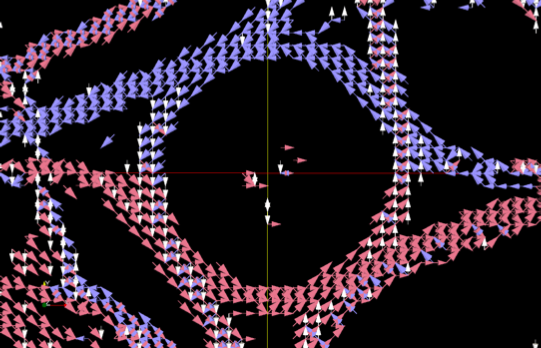
\includegraphics[width=.6\textwidth]{figures/condi_tran_map.png}
    \caption[Conditional transition map of a roundabout.]{Conditional transition map of a roundabout \citep{kucner2013conditional}. Arrows indicate the exit directions for that cell. For simplicity, the entering directions are not drawn. One can see that this model captures how cars drive through the roundabout. }
    \label{fig:condi_tran_map}
\end{figure} 

\subsection{Dynamic Environment Modeling}

For a mobile robot to operate, a proper way to model the environment is necessary. \citet{elfes1989using} introduces occupancy grid as a representation of environment, which divides the environment into a grid of cells with a predefined resolution. Each cell is a random variable with values of either \textit{occupied} or \textit{not occupied}. The occupancy grid assumes the environment being static, which does not hold in real world situations. For example, a robot might need to work in a traffic intense environment with driving cars and pedestrian. 

Early attempts to model dynamics in environment extend occupancy gird with a timescale framework. \citet{arbuckle2002temporal} propose to model dynamics with a stack of occupancy grids with each layer corresponding to a different timescale. They call this representation Temporal Occupancy Grid (TOG). Objects' motion pattern can then be classified based on their occupancy traces across different layers of TOG. For example, if a cell is occupied across all layers of TOG (i.e., occupied at all timescales), it is likely to be a part of the background. Similarly, traffic patterns with various speeds can be identified based on their occupancy traces on a certain layer of TOG. \citet{biber2009experimental} use multiple map representations of the dynamic environment with different timescales for long-term SLAM. Mapping is refreshed based on a sample set of observations that is updated over time by random replacement. Different timescales relates to different learning rate. Map with higher learning rate adapts to new observations faster than these with lower learning rates.

Although the above methods can be applied for modeling dynamics, essentially their static nature remains if we look at each layer that characterizes a specific timescale. In order to capture the dynamic nature of environment, \citet{meyer2012occupancy} propose to model state changes of cells by a two-state hidden Markov models (HMMs). Therefore, the dynamics in environments are explicitly characterized by the state transition probabilities of HMMs. The parameters of these HMMs are estimated with an Expectation Maximization (EM) algorithm. 

However, although their method relaxes the static cell state assumption made by occupancy grid, they assume that state changes of cells are caused by a \textit{stationary} process. In other words, a cell's state transition probabilities are constants over time. Moreover, the assumption of independences between cells is not always valid since state change of a cell's neighboring cells is a strong indicator of that cell's future state. Due to above reasons, cell-specific input-output HMMs (IOHMMs) are used by \citet{wang2014modeling} to better model dynamic environments. An IOHMM imposes conditional dependences on latent variable and observed variable with an input sequence. An illustration of IOHMM used in their method is depicted in Figure \ref{fig:IOHMM}. The input sequence is determined by past observations of neighboring cells. By this way, the transition model of their method is adaptive to input sequence that varies over time, which relaxes the assumption of stationary process made by \citet{meyer2012occupancy}. It also incorporates spatial correlations by making input sequence dependent on neighboring cells. 

\begin{figure}[H]
  \centering
    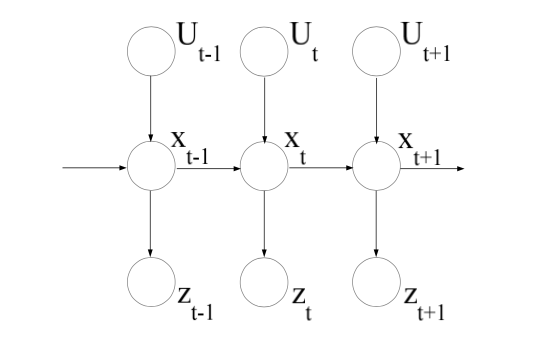
\includegraphics[width=.6\textwidth]{figures/IOHMM.png}
    \caption[An illustration of IOHMM.]{An illustration of IOHMM used by \citet{wang2014modeling}. Note in this IOHMM only latent variables are dependent on input sequence, which is determined by past observations in neighboring cells.}
    \label{fig:IOHMM}
\end{figure} 

Our method is conceptually equivalent to theirs. In both methods, the influence of neighboring cells is captured by conditional dependence. Although our motion model is fixed for a specific map, the occupancies propagate to a certain cell only when its neighboring cells have velocities towards it. This mechanism acts as a ``trigger'' which only get triggered at certain time and essentially makes our model time dependent.


\section{Neural Networks} \label{lr:network}

Since \citet{krizhevsky2012imagenet} applied deep convolutional neural networks (CNNs) in large scale image classification in 2012, CNNs have gained a lot of successes in computer vision. Researches show that the depth of network plays a very important role in CNNs' performance \citep{simonyan2014very}. However, deep networks are more difficult to train, possibly due to poor gradient flow during back-propagation. To address this problem, \citet{he2016deep} propose to fit a \textit{residual} mapping with stacked layers of CNNs instead of fitting the desired underlying mapping directly. This idea is implemented as ``shortcut connections'' between layers. A shortcut connection branches from one layer and connects to one of the followed layers. Moreover, \citet{huang2016densely} extends the idea of residual learning so that each layer has a shortcut connection to every other layer in the network. This design guarantees layers with easy access to its preceding layers and makes feature reuse very easy. Figure \ref{fig:dense_net} shows a five layer densely connected CNN (DenseNet).  Compared with other CNN structures like ResNets, DenseNets are better at alleviating vanishing-gradient problem and therefore improve classification accuracy with even fewer parameters. 

\begin{figure}[H]
  \centering
    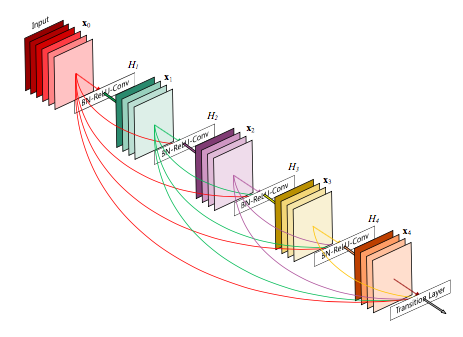
\includegraphics[width=.6\textwidth]{figures/denseNet.png}
    \caption[A five layer dense block.]{A five layer dense block \citet{huang2016densely}. As can be seen, each layer has a shortcut connection to every other follower layer in the network.}
    \label{fig:dense_net}
\end{figure} 

Besides image classification, CNNs have been extensively used in other computer vision tasks like semantic segmentation. Unlike in image classification where only one class has to be determined for the whole image, semantic segmentation requires  classification at pixel level. \textit{Fully} convolutional neural networks have been proposed by \cite{long2015fully} to tackle this problem. By removing fully connected layers and adding a deconvolution layer that functions as upsampling, their network is able to take arbitrary size image as input and predicts pixel-wise classification. Their network also includes skip connections that combine deep coarse features (e.g., semantic information) and shallow fine features (e.g., geometric shape and appearance), both of which are proved to be essential for semantic segmentation. \citet{jegou2017one} extends fully convolutional networks with dense blocks, i.e., a block of convolutional layers that \textit{densely} connected as in DenseNet. Their proposed structure is designed for semantic segmentation, with a downsampling path extracting high-level semantic feature and an upsampling path recovering outputs to full resolution as input image. 

The network structure used in this thesis is similar to that of \citet{jegou2017one}. Since our proposed motion model needs to be place dependent, our network is required to predict probabilities at cell level, which is similar to pixel level prediction in semantic segmentation. The differences lie in the meaning of these probability outputs. For semantic segmentation, these are probabilities of a pixel belonging to a specific semantic class, while in our case they are probabilities of object's exit direction conditioned on which direction it takes to reach current cell.   

As CNNs are good fit for image based tasks, recurrent neural networks (RNNs) are found to be very useful to deal with sequential data such as videos and texts. RNNs have been successfully applied in applications like object tracking \citep{ondruska2016deep}, automatic language translation \citep{cho2014learning} and speech recognition\citep{graves2013speech}. Long short-term memory (LTSM) \citep{hochreiter1997long} addresses vanishing and exploding gradient problems and becomes one of most popular variants of RNNs. 

\begin{figure}[ht]
  \centering
    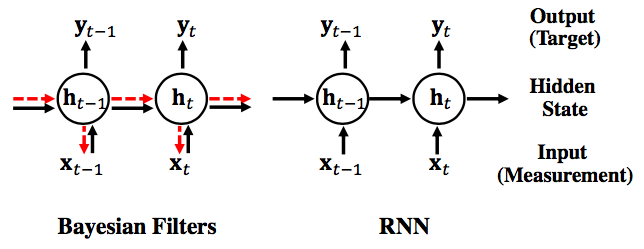
\includegraphics[width=.7\textwidth]{figures/rnn_and_bayes.png}
    \caption[Comparison between RNN and Bayesian filters.]{Comparison between RNN and Bayesian filters \citep{de2017dynamic}. For Bayesian filers, the dynamics are modeled by a Markov process (red dash lines). In both cases, measurements are fed into the systems as inputs.}
    \label{fig:rnn_and_bayes}
\end{figure} 

\citet{ondruska2016deep} propose a framework named \textit{deep tracking} for object tracking with 2D laser data. Deep tracking uses RNNs as the underlying model, and it is designed to be trained in an end-to-end fashion from raw sensor data without hand-crafted feature engineering. Unlike in most supervised learning applications where human annotated ground truth is needed, they train the network with future sensor observations (i.e., future inputs to network) as ground truth, which essentially makes the training unsupervised. Further, \citet{ondruska2016end} extends their deep tracking framework so that it can perform object tracking and semantic segmentation at the same time. 

The fact that object tracking can be achieved by both Bayesian filter based approaches like BOF and RNN based approaches like deep tracking leads us to understand their connections. In a paper that aims at dynamic facial analysis, \citet{de2017dynamic} try to compare Bayesian filters with RNNs as depicted in Figure \ref{fig:rnn_and_bayes}. Given noisy measurement as input, the goal of Bayesian filter is to estimate the hidden state and optionally the target output, while RNNs sequentially predict target output as a function of hidden state which is in turn dependent on new measurements. The performance of Bayesian filters is highly dependent on how much the assumed transition model and measurement model are close to real situations. While for RNNs, this step of handcrafted engineering is avoided since RNNs are able to model them implicitly by learning from data, which is similar to how CNNs extract features from images without artificial feature engineering. On the other hand, despite its successes in many applications, how the hidden states involve over time and how to interpret the hidden states remain a challenge in understanding RNNs. For Bayesian filter, interpretations of the transition processes are usually quite straightforward. 



\cleardoublepage
%!TEX root = ThesisLKN.tex
\chapter{Theoretical Background} \label{chapter:3}

This chapter introduces the theoretical background of this thesis, which mainly concerns two distinct parts: Bayesian Occupancy Filter (BOF) and Convolutional Neural Network. In Section \ref{sec:bayes_filtering}, we start with introduction to the idea of Bayesian filtering. BOF is naturally introduced in Section \ref{sec:bof}, since it is an extension of Bayesian filtering on occupancy grid for object tracking. To better adapt BOF to human tracking context, Section \ref{sec:bofmp} explains how our human motion model can be seamlessly incorporated into the BOF framework. In Section \ref{sec:cnn}, we firstly introduce the general structure of CNNs, and the state-of-the-art densely connected CNNs (DenseNets) are explained in Section \ref{sec:dense_net}. To exploit the power of DenseNets for networks that produce \textit{pixel-wise} predictions , the fully convolutional DenseNets with upsampling path are introduced in Section \ref{sec:fc_dense_net}. 

\section{Bayesian Occupancy Filter} 

In a tracking system, the locations of tracked objects are estimated by taking into accounts both incoming measurements from sensor and predictions from last time step. This process is very similar to Bayesian filtering, which is a probabilistic way to \textit{recursively} estimate the state of a dynamic system.

\subsection{Bayesian Filtering} \label{sec:bayes_filtering}

Bayesian filters work in a dynamic system. At any time $t$, the true state $x_t$ of the dynamic system is unobservable. Instead, measurements $z_t$ can be obtained from sensor data and their relationship can be expresses as \citep{jazwinski2007stochastic}:

\begin{equation}
z_t = h_t(x_t, \omega_t)
\end{equation}

where $h_t$ is known as \textit{observation model}, and $\omega_t$ is \textit{measurement noise}. The true state $x_t$ evolves from last state $x_{t-1}$ based on a \textit{process model} $f_t$:

\begin{equation}
x_t = f_t(x_{t-1}, v_{t-1})
\end{equation}

where variable $v_{t}$ is called \textit{process noise}. This equation describes a \textit{Markov process} with order one, since current state $x_t$ only depends on last state $x_{t-1}$ and does not depend on past states $x_{1:t-2}$ . For a dynamic system, the goal of Bayesian filtering is to recursively estimate the \textit{posterior} probability distribution $P(x_t|z_{1:t})$. This is done in two steps: \textit{prediction} and \textit{estimation}. In the prediction step, a \textit{prior} distribution on the state of the system is calculated based on posterior distribution from last time step and the process model. In the estimation step, the prior distribution is corrected by new measurements to calculate posterior distribution on the current state.

\subsection{BOFUM Formulation} \label{sec:bof}

BOF, similar to Bayesian filer, consists of two stages: \textit{prediction} and \textit{estimation}. Bayesian Occupancy Filter (BOF) can be applied on robots to reason about the dynamic environment, which in this context is represented by occupancy grid. Applications of BOF include collision avoidance \citep{coue2006bayesian} and object tracking \citep{chen2006dynamic}.

Historically, based on different representations of the cell's state space, there are two formulations of BOF: 4D-BOF and 2D-BOF. In 4D-BOF, each cell has four dimensions, with two dimensions representing its position on the grid, and the other two representing the orthogonal velocity components \citep{coue2006bayesian}. While for 2D-BOF, cells are organized as in a 2-dimensional occupancy grid, and each cell is associated with probability distributions of its velocity. The advantage of 4D-BOF is that it is able to represent overlapping objects with different velocities. However, 4D-BOF is more computationally expensive and it is not able to estimate cell's velocity. On the contrary, 2D-BOF dose not allow overlapping objects but requires less computations and is able to infer velocities. In this thesis, we follow the 2D-BOF formulation that is proposed by \citet{gindele2009bayesian}, who extend original 2D-BOF using prior map knowledge (BOFUM) as an indicator for motion preference. 			

We start the formulation of BOFUM by introducing relevant random variables. The subscript $n$ of each random variable represents the cell index on the grid map. We assume there are $N$ cells in total. For time step $t$, we define:

\begin{my_enumerate}
\item[] $O:$ Vector for occupancy state of all cells. Each element $O_n$ takes two possible values, $occ$ and $nocc$.
\[ O = (O_1, \ ... \ , \ O_N)^T \in \{ occ, nocc\}^n \]

\item[] $V:$ Vector for velocities in $x$ and $y$ directions. Velocities are discretized into cells, therefore have unit of $cell/timestep$.
\[ V = (V_1, \ ... \ , \ V_N)^T \in \{ \mathbb{Z}, \mathbb{Z}\}^n \]

\item[] $X:$ Combination of both occupancy and velocity. 
\[ X = (O, \ V) \]

\item[] $X^-:$ Occupancy and velocity state at time $t-1$.
\[ X^- = (O^-, \ V^-) \]

\item[] $R:$ Matrix of random variables describing reachability from cell $a$ to cell $c$. This information is hand-crafted based on cell's context on the grid map. 
\[ R \in \{reach, nreach\}^{n \times n}\]

\item[] $T$: Transition vector. For $T_i = j$, it represents that the occupancy in cell $i$ will move to cell $j$ in the next time step. The transition is an abstraction over velocity, reachability and any other information about the cell movement. 
\[ T = (T_1, \ ... \ , \ T_N)^T \in N^n\]

\item[] $Z$: Measurement vector that comes from sensor data.
\[Z = (Z_O, \ Z_V), Z_O \in  \{ occ, nocc\}^n , Z_V \in \{ \mathbb{Z}, \mathbb{Z}\}^n\]

In our context, we use no sensors for measuring velocities. Therefore, $Z_v$ will be omitted.
\end{my_enumerate}

We assume that cells are independent to each other. This simplifies the formulation and also makes the implementation of BOF highly parallelizable. The goal of BOF is to estimate the posterior probability distribution of the state of a specific cell $c$ given measurement $Z_c$:
\begin{align}
P(X_c|Z_c) &= \frac{P(X_c, Z_c)}{P(Z_c)} \label{eq:1} \\ 
         &= \frac{\sum_{X^-, R, T}{P(X_c, X^-, R, T, Z_c)}}{\sum_{X^-, R, T, X_c}{P(X_c, X^-, R, T, Z_c)}} 
\end{align}
Since $P(Z_c)$ can be obtained by marginalization, i.e., $P(Z_c)= \sum_{X_c}{P(X_c, Z_c)}$, we only concern the numerator of Equation \ref{eq:1}:
\begin{equation}
P(X_c|Z_c) \propto \sum_{X^-, R, T}{P(X_c, X^-, R, T, Z_c)} \label{eq:4}
\end{equation}

In order to calculate joint probability $P(X_c, X^-, R, T, Z_c)$, we need to decompose it based on Baye's rules and some assumptions. 
\begin{align}
P(X_c, X^-, R, T, Z_c) &= P(X_c, X^-, R, T)P(Z_c|X_c, X^-, R, T) \label{eq:3}\\
                     &= P(X_c, X^-, R, T)P(Z_c|X_c) \\
                     &= \underbrace{P(X_c | X^-, R, T) P(X^-, R, T)}_{prediction} \underbrace{P(Z_c|X_c)}_{correction} \label{eq:2}
\end{align}

So far, the two main stages of Bayesian filtering can been identified by Equation \ref{eq:2}: 

\begin{my_enumerate}
\item \textbf{prediction}: The prediction step calculates a prior distribution of the state of cell $X_c$, which is joint distributed with past state $X^-$, reachability $R$ and transition $T$. It can be further decomposed as in Equation \ref{eq:2}. 

$P(X_c | X^-, R, T)$ specifies the \textit{process model}, which states how the current state can be predicted given a prior state and extra knowledge. Since occupancy and velocity are independent and transition subsumes velocity and reachability, we have
\begin{equation}
P(X_c | X^-, R, T) = P(O_c|O^-, T)P(V_c|O^-, T)
\end{equation}
For the propagation of occupancy, we assume that it is sufficient for a cell $c$ to be occupied, if at least one antecedent cell $a$ moves to cell $c$. This assumption can be expressed as:
\begin{align}
P(O_c=occ|O^-, T) &= 
  \begin{cases}
  1, & \vee_{a \in N} ((O_a=occ) \wedge (T_a=c)) \\
  0, & else
  \end{cases} 
\end{align}
For simplicity of implementation, we calculate `$nocc$' instead of calculating `$occ$':
\begin{align}
P(O_c=occ|O^-, T) &= 1 - P(O_c=nocc|O^-,T) \\
                  &= \prod_{a \in N}{(1-P(O_c=occ|O^-_a,T_a))}
\end{align}
where 
\begin{equation}
P(O_c=occ|O^-_a, T_a) =
  \begin{cases}
  1, & (O_a=occ) \wedge (T_a=c) \\
  0, & else
  \end{cases} 
\end{equation}

For an antecedent cell $a$ that moves to cell $c$, the propagation of velocity is expressed as:
\begin{equation}
P(V_c=v(a, c)| O^-, T) = P(O_c=occ|O^-_a, T_a) \label{eq:6}
\end{equation}
where $v$ is helper function that expresses velocity from cell $a$ to cell $c$.

$P(X^-, R, T)$ is the joint distribution for transition. By assuming occupancy and transition are independent, we have
\begin{align}
P(X^-, R, T) &= P(O^-, V^-, R, T) \\
             &= \prod_{i \in N} P(O_i^-) \prod_{j \in N} P(T_j, V^-, R)
\end{align}
Since we assume \textit{Occupancy preservation}, occupancy of an antecedent cell $a$ must propagate to follower cells $m$. This introduces a normalization coefficient $\mu$:
\begin{align}
P(T_a=c, V^-, R) &= \frac{P(T_a=c, V^-_a, R_{a,c})}{\sum_{m \in N}P(T_a=m, V^-_a, R_{a,m})} \\
                 &= \mu_a P(V_a^-) P(R_{a,c})P(T_a=c|V_a^-, R_{a, c}) \label{eq:t}
\end{align}
where 
\begin{equation}
P(T_a=c|V^-_a, R_{a,c}) =
  \begin{cases}
  1, & V_a^- = v(a, c) \wedge (R_{a,c} = reach) \\
  0, & else
  \end{cases} 
  \label{eq:t1}
\end{equation}

\item \textbf{estimation}: The estimation step multiplies a prior distribution calculated from \textit{prediction} with a conditional probability distribution that represents \textit{correction} based on an \textit{observation model}. We do not use any sensor for measuring velocity, and we assume cell's occupancy state can be extracted from raw sensor data after preprocessing. The observation model captures the uncertainty involved in sensor measuring given cell's occupancy state:
\begin{align}
P(Z_{O,c}=z_c|X_C) &= P(Z_{O,c}=z_c|O_C) \\
				   &=
				   \begin{cases}
				   1-\omega_Z, & z_c = o_c \\
				   \omega_Z,   & else
				   \end{cases}
\end{align}
where $\omega_Z \in [0,1]$ and higher its value, less confident we are in the measurements. 
\end{my_enumerate}

\begin{figure}[ht]
  \centering
    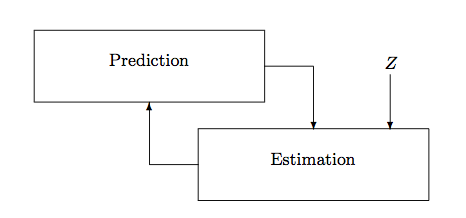
\includegraphics[width=.6\textwidth]{figures/bof_recursive.png}
    \caption[The prediction and estimation loop of BOF.]{The prediction and estimation loop of BOF \citep{tay2008bayesian}}
    \label{fig:bof_recursive}
\end{figure} 

To summarize, the \textit{prediction} and \textit{estimation} steps of BOF work recursively as shown in Figure \ref{fig:bof_recursive}. To calculate posterior probability distribution $P(X_c|Z_c)$, we need firstly calculate the joint distribution in Equation \ref{eq:4} as:
\begin{align}
\sum_{X^-, R, T}P(X_c, X^-, R, T, Z_c) &= P(Z_c|O_c) \sum_{O^-, V^-, R, T}P(V^-,R,T)P(O^-)P(O_c|O^-,T)P(V_c|O^-,T) \notag  \\
                        &= P(Z_c|O_c) \sum_{O^-, T}P(T)P(O^-)P(O_c|O^-,T)P(V_c|O^-,T) \notag \\
                        &=  \underbrace{P(Z_c|O_c)}_{correction} \notag \\
                        & \ \ \ \ \underbrace{\sum_{O^-, T}P(T)P(O^-)P(O_c|O^-,T)}_{occupancy \ prediction} \label{eq:occ_pred} \\
                        & \ \ \ \ \underbrace{\sum_{O^-, T}P(T)P(O^-)P(V_c|O^-,T)}_{velocity  \  prediction} \label{eq:vel_pred}
\end{align}

As can be seen from above equations, $P(T)$ is needed for prediction. Based on Equation \ref{eq:t} and \ref{eq:t1}, we have:
\begin{align}
P(T_a = c) &= \sum_{V^-, R}{\mu_a P(V_a^-)P(R_{a,c})P(T_a=c|V_a^-, R_{a,c})} \\
		   &= \mu_a P(V_a^-=v(a,c))P(R_{a,c}=reach)
\end{align}

Based on Equation \ref{eq:6} and \ref{eq:vel_pred}, velocity prediction can be derived as:
\begin{align}
P(\hat{V_c}=v(a, c)) &= \sum_{O^-, T}P(T)P(O^-)P(\hat{V_c}=v(a,c)|O^-,T) \\
  &= P(O_a^-=occ)P(T_a=c) \label{eq:infer_velocity}
\end{align}

We then apply uncertainty in acceleration on the predicted velocity $\hat{V}$. The acceleration noise is assumed to be normal distribution with zero mean and covariance $\Sigma$. Therefore the final velocity is predicted as:
\begin{equation}
P(V_c) = \sum_{\hat{V_c}}{P(V_c|\hat{V_c})P(\hat{V_c})} \label{eq:adding_noise}
\end{equation}
where
\begin{equation}
v_c = \hat{v_c} + \omega_a \Delta t, \ \omega_a \sim \mathcal{N}(0, \Sigma) \label{eq:adding_noise}
\end{equation}

For occupancy prediction, the probability of a cell being \textit{not} occupied is firstly calculated. It is easier to calculate since only one case needs to be considered, namely when all possible antecedent cells do not move to that cell.
\begin{align}
P(O_c=nocc) &= \sum_{O^-, T} P(O^-)P(T)P(O_c=nocc|O^-,T) \\
            &= \sum_{O^-, T}\prod_{a \in N} P(O_a^-)P(T_a)P(O_c=nocc|O^-_a,T_a) \\
            &= \prod_{a \in N} \sum_{O_a^-, T_a} P(O_a^-)P(T_a)P(O_c=nocc|O^-_a,T_a) \\
            &= \prod_{a \in N} (1-P(O_a^-=occ)P(T_a=c))
\end{align}
Therefore, the probability of a cell being occupied can be calculated as:
\begin{align}
P(O_c=occ) &= 1 - P(O_c=nocc) \\
           &= 1 - \prod_{a \in N}{(1-P(O_a^-=occ)P(T_a=c))}
\end{align}

\subsection{BOF with Motion Pattern (BOFMP)} \label{sec:bofmp}

In the above formulation of BOFUM, if we do not consider acceleration noise and occupancy propagates from an antecedent cell $a$ to cell $c$ with velocity $v(a,c)$, cell $c$ will propagate the occupancy with the same velocity $v(a,c)$. In other words, BOFUM assumes a constant velocity motion model with uncertain zero-acceleration. In reality, object actually follows motion patterns based on its location on the map. For example, a car driving on a lane are more likely to drive along the lane instead of driving to sidewalks. To capture this intuition, \citet{gindele2009bayesian} incorporate motion preference into the reachability matrix $R$.

For a cell $c$ on the occupancy grid, they assign a terrain type for each cell with a helper function $u$. In their automotive application, they define three terrain types: $U=\{lane, sidewalks, unknown\}$. The reachability probability between cell $a$ and cell $c$ can be calculated as:
\begin{equation}
P(R_{a,c}=reach) = S_{u(a), u(c)} \omega(a, c) \label{eq:reachability}
\end{equation}
where matrix $S\in[0,1]^{U\times U}$ defines the likelihood of change terrain types, and $\omega: N \times N \rightarrow [0,1]$ captures the likelihood of the movement when both cells are in the same terrain type or when the distance between these two cells has influence on the likelihood.

However, their way of modeling place dependent motion patterns has two disadvantages: 1) Manually classifying terrain types might be reasonable in their automotive applications, but it is not feasible in our human tracking scenarios. Although indoor environments, like offices and factories, can be classified as \textit{walkable} or \textit{not walkable}, this kind of classification provide too less information on motion preference. 2) As shown in Equation \ref{eq:reachability}, the $S$ matrix and weight function $\omega$ have to be manually defined. When an object is being tracked, the environment is updated rapidly, which requires to update the reachability matrix with a high frequency. Besides, when large maps are considered, it requires a lot of manual work to define function $\omega$ since any two cells on the grid map have to be considered. Therefore, defining reachability is very time consuming and inflexible. 

To deal with the mentioned disadvantages, we propose to model motion patterns in a \textit{learning-based} way. Although we apply this method only on modeling human motion patterns in indoor environment, it can be also used in other scenarios, such as modeling car motion pattern in outdoor environment. The idea is to train a neural network based on relevant data extracted from human trajectories. Once the network finished training, it learns the implicit motion patterns that are imposed on the human trajectories used for training. For a given grid map, the network is able to output data that can be interpreted as motion patterns without human intervention. This facilitates its application in real scenarios even with rapidly changing environments.   

The relevant data we extracted from human trajectories can be used as an proxy of human motion patterns. They are represented as a set of conditional probabilities for every cell on the map. They represent how likely a person moves to one of the neighboring cells (exit direction), conditioned on which neighboring cell he or she comes from (entering direction). Mathematically, for any cell $c \in [1,N]$ on the grid map, they can be expressed as
\begin{equation}
P_c(V^{ex}|V^{en}) 
\end{equation}
where $V^{ex}, V^{en}$ represent exit and entering direction respectively, and $V^{ex}, V^{en} \in \{U, L, R, D, DL, DR, UL, UR\}$ \footnote{U: up, L: left, R:right, D:down}.
Since these probabilities incorporate information about the incoming cell, the motion model captures \textit{spatial correlations} between cells. Besides, they are different for each cell based on cell’s context on the map, which means the learned motion pattern is expressive enough to predict different motions at different locations. In other words, our motion model is also \textit{place dependent}.

Figure \ref{fig:condi_prob_example} shows an example of how our model captures motion preference based on its location on the map. A person is currently at the location indicated by the green rectangle and arrives by taking entering direction of left. The most possible exit directions, as shown by red arrows in the left plot, show that this person is likely going either up-left or down-left in the next time step. This is expected since we can infer no bias towards either of the directions from the symmetric map. The motion model for the cell related to that location is represented by conditional probabilities shown in the right plot. It only shows $P_c(V^{ex}|V^{en}=L)$.
\begin{figure}[ht]
  \centering
    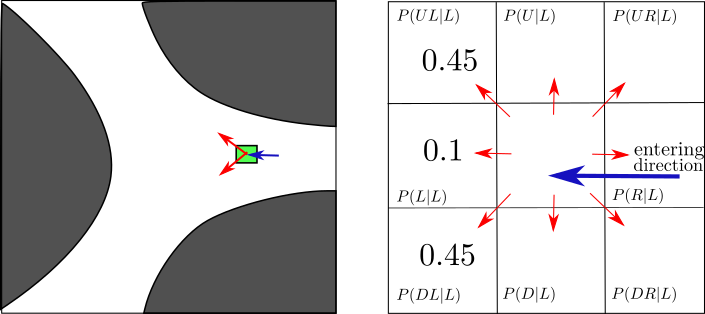
\includegraphics[width=.85\textwidth]{figures/bofmp_example.png}
    \caption[An example of our proposed motion model.]{An example of our proposed motion model. \textbf{LEFT}: A person is at location indicated by the green rectangle. White area is walkable. The blue arrow and red arrows show entering and exit directions. \textbf{RIGHT}: The motion pattern at that cell represented as $P_c(V^{ex}|V^{en}=L)$. It shows that, for the next time step, this person is more likely to turn either up-left or down-left than keep going left.}
    \label{fig:condi_prob_example}
\end{figure}

The way how we incorporate our motion model into BOFUM similar to adding acceleration noise to predicted velocity in Equation \ref{eq:adding_noise}. After the inferred velocity $\hat{V}$ is calculated based on process model as shown in Equation \ref{eq:infer_velocity}, the final velocity is calculated as:
\begin{equation}
P(V_c) = \sum_{\hat{V_c}}{P_c(V^{ex}=V_c|V^{en}=\hat{V_c})P(\hat{V_c})} \label{eq:motion_pattern}
\end{equation}
where $P_c(V^{ex}|V^{en})$ is \textit{cell-specific} motion pattern. In this ways, the BOFMP knows how to propagate occupancies according to human motion pattern at certain locations. When compared with BOFUM, this method leads to better tracking performance especially when no observations are given or in occluded scenarios.

In this section, we assume the maximum velocity of the object is 1 $cell/timestep$. In reality, the objects may perform higher velocities. However, the neural network used for extracting motion pattern only models velocity of 1 $cell/timestep$. The method of how we adapt the extracted motion model to higher velocities will be explained in Section \ref{sec:BOFMP_implementation}.

\section{Convolutional Neural Network} \label{sec:cnn}

Neural networks are mathematical abstraction about how our human nervous system process and learn from data. Over the last few years, neural networks have been extensively used in many applications, such as computer vision \citep{russakovsky2015imagenet}, natural language processing \citep{cho2014learning} and robotics \citep{levine2016learning}. Neural networks are organized as a layered structure, which replicates forward flow of information through human nervous system. Each layer consists of a certain number of \textit{neurons}. In regular neural networks, those layers are \textit{fully} connected. That is, neurons between two adjacent layers are pairwise connected, but neurons within a single layer have no connections with each other. For a single neuron, assuming its inputs are expressed by a vector $\mathbf{x}$, its parameters are weights $\mathbf{w}$ and bias $b$, and its output is a scalar value:
\begin{equation}
y = f(\mathbf{w}^T \mathbf{x} + b)
\end{equation}
where $f$ is a non-linear function, which is known as \textit{activation function}. Popular choices for activation function include:

\begin{my_enumerate}
\item \textbf{Sigmoid function}: $f(x)=\frac{1}{1+e^{-x}} \in [0, 1]$. One undesired property of sigmoid function is that it gets saturated at both ends, which means the gradient for very small or very large inputs are almost zeros. In other words, sigmoid function ``kills'' gradient which may affect training of networks. 
\item \textbf{Tanh function}: $f(x)=\frac{e^x-e^{-x}}{e^x+e^{-x}} \in [-1, 1]$ Similar to sigmoid function, tanh function also saturates and ``kills'' gradients. However, its output is zero-centered.
\item \textbf{ReLU}: $f(x)=max(0, x) \in [0, +\infty)$. ReLU never saturates and this may accelerate convergence of network training as shown in \cite{krizhevsky2012imagenet}. Variants of ReLU include leaky-ReLU and PReLU \cite{he2015delving}.
\end{my_enumerate}

To train a neural network, ground truth must be given since neural network is a supervised learning algorithm. Besides, a \textit{loss function} has to be defined in order to measure how close are our network predictions to the ground truth. Commonly used loss functions are cross-entropy loss for classification and L2 squared norm for regression. Based on the loss calculated for training data, the network has to be optimized in terms of finding the best parameters of the network so that the loss is minimized. It turns out that following the (reversed) direction of gradients of the loss function is an effective way to update these parameters. Based on this observation, many optimization algorithms for neural networks have been proposed, such as Stochastic Gradient Descent (SGD), RMSProp and Adam (see more in \cite{ruder2016overview}). 

Convolutional Neural Networks (CNNs) are a special kind of neural network that works well with image data. In regular neural networks, the neurons for each layer is organized as a one-dimensional vector. While for CNNs, they are arranged in three dimensions: width, height and depth. For the input layer (i.e, the first layer), width and height are the spatial dimensions of an image and depth corresponds to the RGB channels of a color image. For image classification, the output layer is $1\times1\times N$ dimensional, with N corresponding to number of classes. CNNs are also organized as a stack of layers, and the most common layers are:

\begin{my_enumerate}
\item \textbf{Convolutional Layer} (CONV): The core layer of a CNN. CNNs learn the complex structure in image data by firstly extracting useful features, such as edges or a blotch of some color in shallow layers and semantic wheel-like or nose-like features in deeper layers. Those features are extracted by applying filters on 3D volume of data on each layer and this process is represented by a CONV layer. CONV layer utilizes \textit{local connectivity}, which means they extract feature only on a local region of the input data. Thanks to its \textit{parameter sharing} scheme, the number of parameters in CONV layers are much less than in layers of a regular neural network. The output volume of CONV layer depends on three hyperparameters: depth, stride and zero-padding.
\item \textbf{ReLU Layer} (RELU): This layer introduces non-linearities to the network and work as activation function as in regular neural networks. It applies ReLU function point-wise on the input volume.
\item \textbf{Pooling Layer} (POOL): This layer works as a downsampling operation that reduces the size of input data and ensures spatial invariance to some degrees. Typical pooling operation include max pooling and average pooling.
\item \textbf{Fully-connected Layer} (FC): As its name indicated, each of the neuron in FC layer is connected to all neurons in its preceding layer as in regular neural networks. For image classification tasks, the last layer is normally a FC layer. 
\item \textbf{Batch-Normalization Layer}(BN): Batch normalization is a technique that has been proposed in \citep{ioffe2015batch} to address the so-called internal covariate shift phenomena in network training. Using BN layers allows higher learning rate and makes network less sensitive to initialization. 
\end{my_enumerate}

As an example, a simple CNN that used for image classification can be expressed as:
\begin{equation*}
\text{INPUT}\rightarrow[\text{CONV}\rightarrow \text{BN} \rightarrow \text{RELU} \rightarrow \text{POOL}] * 2 \rightarrow \text{FC}
\end{equation*}

\subsection{Densely Connected Convolutional Networks } \label{sec:dense_net}

In the development of CNNs, \citet{Simonyan14c} show that the depth of CNNs plays an very important role in its performance. However, the experiments from \citet{he2016deep} show that with increased depth, the accuracy of network predictions firstly gets saturated and then degrades rapidly. In theory, the deeper network should perform at least as good as its shallower counterpart, because the redundant layers can at least learn an identity mapping, i.e., directly produce input as output. This unexpected performance degradation leads to their conclusion that CNNs are not good at learning identify mapping. To address this problem, they propose \textit{residual} learning. Assume the underlying desired mapping that represented by few stacked layers is $\mathcal{H}(\mathbf{x})$. Instead of learning it directly, its residual,
\[\mathcal{F}(\mathbf{x}) = \mathcal{H}(\mathbf{x}) - \mathbf{x}\]
is learned and a \textit{skip connection} is connected from the input to the output of these stacked layers. Therefore, the final learned mapping is $\mathcal{F}(\mathbf{x}) + \mathbf{x} = \mathcal{H}(\mathbf{x})$. This idea is illustrated in Figure \ref{fig:res_idea}. 
\begin{figure}[ht]
  \centering
    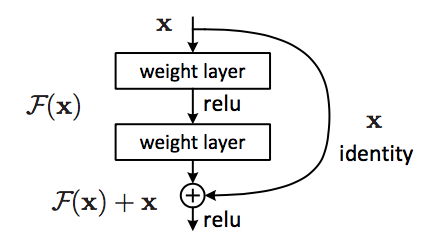
\includegraphics[width=.55\textwidth]{figures/res_idea.png}
    \caption[An illustration of residual learning]{An illustration of residual learning \citep{he2016deep}. Instead of fitting the desired underlying mapping directly, a residual mapping $\mathcal{F}(\mathbf{x})$ is learned with few stacked layers.}
    \label{fig:res_idea}
\end{figure}

The advantages of residual learning is that it facilitates the gradient flow from deep layers to shallow layers through the skip connection. We define a composite function $H_l(\cdot)$ that can be represented by a few stacked layers such as BN, POOL, RELU and CONV. $l$ is the layer index. Therefore, for the input $\mathbf{x}_{l-1}$, the output of residual learning from layer $l$ is:
\begin{equation}
\mathbf{x}_{l} = H_l(\mathbf{x}_{l-1}) + \mathbf{x}_{l-1}
\end{equation}
\citet{huang2016densely} propose a similar network structure that heavily uses skip connections. To encourage \textit{feature reuse}, they concatenate feature maps from all preceding layers $0, \ldots, l-1$, which are then used as input of current layer $l$:
\begin{equation}
\mathbf{x}_{l} = H_l([\mathbf{x}_{0}, \mathbf{x}_{1}, \ldots, \mathbf{x}_{l-1}]) 
\end{equation}

A block of $L$ layers that are densely connected in such a way is called as a \textit{dense block}, and it has $\frac{L(L+1)}{2}$ connections. On example of a five layer dense block is shown in Figure \ref{fig:dense_net}. This special design of DenseNet leads to its state-of-the-art performance in image classification tasks.

\subsection{Fully Convolutional DenseNet} \label{sec:fc_dense_net}

The regular CNN are designed for image classification, where only one vector of class scores is needed from network output. In some other tasks such as semantic segmentation, every pixed has to be classified into a certain class, i.e., the output must have the same spatial resolution as input image. This cannot be achieved by regular CNNs, since pooling operations are essential in networks but they also reduce spatial extent.

To achieve classification at pixel level, fully convolutional neural networks (FCNs) have been proposed by \citet{jegou2017one}. By using only convolutional layers and \textit{deconvolution} layers that functions as upsampling, their network is able to take arbitrary size image as input and predicts pixel-wise classification. A deconvolution operation is essentially \textit{backward} convolution. Deconvolution, compared with interpolation, is a natural choice for upsampling in CNNs since it is learnable and thus facilitates end-to-end learning of the networks. How downsampling and upsampling is achieved in CNNs is illustrated in Figure \ref{fig:sampling}

\begin{figure}[ht]
  \centering
    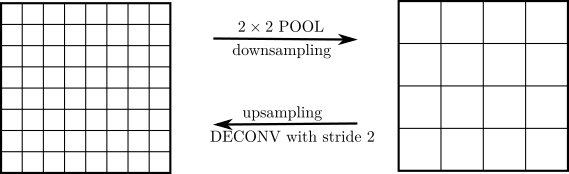
\includegraphics[width=.75\textwidth]{figures/sampling.png}
    \caption[Downsampling and upsampling in FCNs.]{Downsampling and upsampling in FCNs. Left represents a data volume with spatial size of $8\times8$. Downsampling with $2\times2$ pooling operation reduces its size to $4\times4$. Upsamping with deconvolution of stride 2 resumes its size.}
    \label{fig:sampling}
\end{figure}

\citet{jegou2017one} extends fully convolutional networks with dense blocks. Their proposed structure has a downsampling path extracting high-level semantic feature and an upsampling path recovering outputs to full resolution as input image. Their network structure, with some modifications, is used in thesis to extract motion patterns from static maps. As described in Section \ref{sec:bofmp}, we represent motion patterns as cell-specific conditional probabilities $P_c(V^{ex}|V^{en})$. Instead of predicting classification scores, the last layer of our network predicts $8\times8=64$ entries, which are interpreted as eight conditional probability distributions $P_c(V^{ex}|V^{en}=v)$. Each of these conditional probability distributions corresponds to one of eight entering directions. 


\cleardoublepage
%!TEX root = ThesisLKN.tex

\chapter{Implementation Details} \label{chapter:4}

In this chapter, the details on implementations will be described. In detail, how the ground truth data used for training network are generated from simulated human trajectories is described in Section \ref{sec:traj_sim}. In Section \ref{sec:training}, the details on training CNNs are provided. Section \ref{sec:BOFMP_implementation} introduces the code structure of implementing BOFMP. Finally, hyperparameters in the BOFMP tracking algorithm are introduced in Section \ref{sec:hyperparameter}.

\section{Human Trajectory Simulation} \label{sec:traj_sim}

Neural networks are able to capture complex structures in data. For this reason, we train a neural network so that it can be used to extract human motion patterns from static maps. In order to make the network generalizes well, a large amount of human trajectory data in different indoor environments are needed. However, recording human trajectories with 2D laser scans in various indoor environments is expensive, since the hardwares have to be transported to different locations. Besides, since our model requires cell-specific motion patterns, the recorded human trajectories need to cover each discretized cell on the gird map. Even if it is feasible, this requires a lot of time for the laser scanner to work. To collect such a huge amount of real human trajectories is obviously out of the scope of this thesis. As a workaround, we simulated human trajectories on real-world SLAM-generated maps and those simulated trajectories are used for extracting human motion patterns. To validate our method, we evaluate our tracking algorithm on data recorded from real world. 

The maps on which human trajectories are sampled from are floor plans of indoor environments such as laboratories and offices. We assume that human motions in these environment are only constrained by the spatial configurations. Other factors, such as time, social forces and different functional areas, are not modeled. In total, we simulate human trajectories on eight maps, with a total free space area of more than \( 6.6\times10^3 \, m^2 \). Two of those eight maps are shown in Figure \ref{fig:maps}. Each pixed of the map represents a cell on its corresponding occupancy grid, and has resolution of $0.2$ $m/pixel$.

\begin{figure}[ht]
  \centering
    
\includegraphics[width=.8\textwidth, height=.3\textwidth]{figures/map1.png}
    
\includegraphics[width=.8\textwidth, height=.3\textwidth]{figures/map2.png}
    \caption[Two example maps on which human trajectories are sampled from.]{Two example maps on which human trajectories are sampled from. White areas are walkable, and black areas are desks or walls that human cannot walk through.}
    \label{fig:maps}
\end{figure} 

We use A* algorithm to calculate human trajectory between two points on a map. The A* algorithm is a well-know algorithm for path planning. In each iteration of its main loop, A* algorithm decides which step to take based on the summation of two values: one value represents the cost from start to current node and the other represents a heuristic estimate of cost from current node to the goal. The path found by A* algorithm replicates human trajectory, since people normally have a clear goal location in their mind (thus a heuristic estimation) and take a path that requires least efforts to reach it. To account for the fact that human tend to walk some distances away from an obstacle (e.g., people walk in the middle areas of a corridor, which are distant to walls on both sides), we apply two Gaussian filters with different widths on the static maps to get cost maps.  

The actual process from sampling trajectories to obtaining conditional probabilities as motion patterns are implemented in three steps:

\begin{my_enumerate}
\item Sampling trajectories on the full map. In order to get motion dynamics at all possible locations, we sample a predefined number of trajectories with every empty cell on the map as start location. The goal location for each trajectory is randomly sampled but the distance between start location and end location must be within a predefined range. After the start and goal location are defined, a trajectory is calculated by A* algorithm.
\item Calculate probabilities based on trajectories. A \textit{transition} is defined in this context as a person moves from cell $a$ to $c$ through $b$, i.e., $a \rightarrow b \rightarrow c$, where $a$ and $c$ are neighboring cells of $b$. If we consider eight neighboring cells, for each cell it has $8\times8=64$ different transitions. A helper function $v(c_1,c_2)$ is also defined to calculate the velocity from cell $c_1$ to $c_2$. Assume a cell $c$ is identified by its coordinates on $x$, $y$ axis, i.e, $pos(c)=(c_x, c_y)$, then
\[v(c_1, c_2)=\frac{pos(c_2)-pos(c_1)}{\Delta t}\]
Firstly a tensor $C$ is initialized to store these transition counts. So far, Tensor $C$ has 6 dimension of $32\times32\times3\times3\times3\times3$, with first two dimensions representing spatial size of a map window, next two dimensions representing $V^{en}$ and last two dimensions representing $V^{ex}$. For example, for transition $a \rightarrow b \rightarrow c$, we increment the following entry of $C$:
\[ C(pos(b), v(a, b), v(b, c))\]
For each sampled trajectory, we add every transition along this trajectory to its corresponding entry in $C$. The conditional probability $P_i(V^{ex}|V^{en})$ is then calculated from transition counts tensor $C$ as:
\begin{equation}
P_i(V^{ex}=v_1|V^{en}=v_0) = \frac{C(pos(i), v_0, v_1)}{\sum_{ v}C(pos(i), v_0, v)}
\end{equation}
\item Sampling map window with fixed size and data augmentation. The map window that we feed into our network is of size $32\times32$ cells (i.e., $6.4 \times 6.4$m). Therefore, we randomly crop a predefined number of map windows from the whole map. If a map window has free space less than $50\%$, it is not used. To increase the number of data samples, each map window is augmented eight times: for both the map window and its horizontal mirroring, they are rotated by $90^\circ$, $180^\circ$ and $270^\circ$. 

  So far, the ground truth of each map window has same dimensions as $C$, i.e, $32\times32\times3\times3\times3\times3$. However, since the output of network has at most three dimensions, the ground truth has to be resized to $32\times32\times64$, without considering velocity $v=(0, 0)$.
\end{my_enumerate}

The above algorithm is described in Algorithm \ref{algo:data_generation}. 

\begin{algorithm}
\caption{Algorithm for generating data for neural network.}
\label{algo:data_generation}
\begin{algorithmic}[1]
\Procedure{SamplingTrajectories(map, n)}{}
\State $allTrajectories \gets \emptyset$
\For{\textit{cell} in \textit{emptyCells(map)}} 
    \Comment loop over all empty cells on map
	\State $trajectories \gets \emptyset $
	\State $tries \gets 0$
	\While{$tries < N $} 
	\Comment try to sample $N$ trajectories for each cell
	\State $start \gets cell$
	\State $goal \gets sampleGoalLocation(map, start)$
	\State $trajectory \gets AStar(start, goal)$
	\If {$isValid(trajectory)$} 
		\Comment check whether $trajectory$ is empty
		\State \textbf{add} $trajectory$ \textbf{to} $trajectories$
	\EndIf
	\State $tries \gets tries+1$
	\EndWhile
	\State \textbf{append} $trajectories$ \textbf{to} $allTrajectories$
\EndFor
\State \Return $allTrajectories$
\EndProcedure
\\
\Procedure{GetConditionalProbs(Trajectories)}{}
\State Initialize $C$ with zeros
\For{\textit{trajectory} $(c_1, \cdots, c_n)$ in \textit{trajectories}} 
    \Comment loop over all sampled trajectories
    \For{$t=2:n-1$}
    \Comment add transition $c_{t-1} \rightarrow c_t \rightarrow c_{t+1}$
	\State  $idx \gets (pos(c_t), v(c_{t-1}, c_t), v(c_t, c_{t+1}))$
	\State $C(idx) \gets C(idx)+1$ 
    \EndFor
\EndFor
\State $probs \gets calculateProbs(C)$
\State \Return $probs$
\EndProcedure
\\
\Procedure{CropMapWindow(map, probs, S)}{}
\State $data \gets \emptyset$ 
\State $count \gets 0$
\While{$count < S$}
	\Comment try to get $S$ samples
    \State $loc \gets sampleRandomLocation(map)$
    \State $window \gets getWindow(map, loc)$
    \If {$freeSpace(window) < 0.5$}
    	\State \textbf{continue}
    \EndIf
    \State $probWindow \gets getProbWindow(probs, window)$
    \State \textbf{add} $(window, probWindow)$ \textbf{to} $data$
    \State \textbf{add} $agument(window, probWindow)$ \textbf{to} $data$
    \State $count \gets count+1$
\EndWhile

\State \Return $data$
\EndProcedure
\end{algorithmic}
\end{algorithm}

\section{Architecture of Neural Network} \label{sec:training}

As described in Section \ref{sec:cnn}, our network architecture is similar to that of \citet{jegou2017one}, with a minor difference in the last layer (i.e., the output layer). For their use in semantic classification, the input $\mathbf{v}$ to the last year has dimensions of $W\times H \times N$. The first two dimensions are spatial size of the input image, and last dimension corresponds to number of semantic classes. The last layer, known as spatial softmax layer, applies the following function.
\[\varphi(\mathbf{v})_{x, y, j} = \frac{e^{\mathbf{v}_{x, y, j}}}{\sum_{n=1}^N e^{\mathbf{v}_{x, y, n}}}\]
In other words, the output of last layer are class scores that can be interpreted as probabilities. In our case, since the network has to output conditional probabilities $P_c({V^{ex}|V^{en}})$ for all possible $V^{en}$, there are essentially eight probability distributions existing in $\mathbf{v}$. Therefore, our last layer has to firstly segment values to its corresponding $V^{en}$, then apply softmax accordingly. 

\begin{figure}[H]
  \centering
    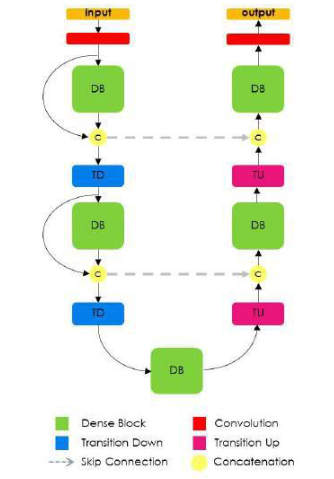
\includegraphics[width=.45\textwidth]{figures/tiramisu.png}
    \caption[Illustration of the fully convolution DenseNet.]{Illustration of the fully convolution DenseNet in \citep{jegou2017one}. The network consists of a downsampling path extracting high-level semantic features and an upsampling path recovering outputs to full resolution as input image. The skip connections, as indicated by dashed lines, combines both deep coarse features and shallow fine features.}
    \label{fig:tiramisu}
\end{figure}

The overall architecture of the network is depicted in Figure \ref{fig:tiramisu}, and how each component is structured is summarized in Table \ref{table:components}. For the network that we use in this thesis, it has 31 convolutional layers, 13 in the downsampling path, 5 in the bottleneck dense block, and 13 in the upsampling path. Two max pooling layers are used to downsample the spatial size of inputs, and two deconvolution layers are used to recover outputs' resolution. Each dense block consists of 5 layers. One important parameter for dense block is the \textit{growth rate}, which is the number of feature maps in each layer. We use a growth rate of 12. Thus, the output of each dense block has $5 \times 12 = 60$ feature maps. The number of feature maps at the end of blocks is listed in Table \ref{table:number_feature_maps}. The network has in total 448,648 parameters.

\begin{table}[H]
\centering  
\begin{tabularx}{.9\textwidth}{c|c}
    \hline
    Component            & Structure            \\ \hline \hline
    Transition Down (TD) & BN $\rightarrow$ RELU $\rightarrow$ $1 \times 1$ CONV $\rightarrow$ $2 \times 2$ MAXPOOL \\ \hline
    Transition Up (TU)   & $3 \times 3$ DECONV with stride 2 \\
   \hline
   Layer                 & BN $\rightarrow$ RELU $\rightarrow$ $3 \times 3$ CONV \\ \hline
   Dense Block (DB).     & 5 Layers that are densely connected \\ \hline
  \end{tabularx}
\caption{Structure of each component in Figure \ref{fig:tiramisu}.}
\label{table:components}
\end{table}

\begin{table}[H]
\centering  
\begin{tabularx}{.53\textwidth}{c|c}
    \hline
    Blocks            & Number of feature maps            \\ \hline \hline
    Input                &    1 \\ \hline
    CONV + DB + C        &    68 \\ \hline
    TD + DB + C          &    128 \\ \hline
    TD                   &    128 \\ \hline
    DB + TU + C          &    188 \\ \hline
    DB + TU + C          &    128 \\ \hline
    DB + CONV            &    64 \\ \hline
    Softmax           &    64 \\ \hline
  \end{tabularx}
\caption{Number of feature maps at the end of blocks.}
\label{table:number_feature_maps}
\end{table}

\newpage
\section{Preprocessing of Tracking Data}

To evaluate our method, we apply the BOFMP filter on real data that are recorded by laser scanners. The real data records occupancy information on a static map which changes over time. Since occupancy indicates a person's location on the map, the time-varying occupancy is able to represent human trajectories. We define the real data that records occupancy information on a given map window for a certain amount of time as a \textbf{scene}. After preprocessing, each scene records human trajectories on that map window so that we can evaluate our method on. However, due to various reasons, such as localization error of robots and discretization errors, the real data could be very noisy. Therefore, a preprocessing pipeline is proposed. It consists of following steps:

\begin{my_enumerate}
\item \textbf{Downsample}. The real data are recorded by laser scanners with frequency of 12Hz, which means we get 12 frames of data per second. Human walking speed in office is roughly 1$\sim$1.2 $m/s$. Since the map resolution is 0.2 $m$, this means for moving one cell in map it takes roughly 2$\sim$2.4 frames. Therefore, We decide to downsample real data by merging the occupancy in 3 continuous frames to 1 frame.
\item \textbf{Remove static occupancy}. A scene is supposed to show the \textit{dynamic} changes of occupancy which represent human trajectory. Therefore, if a cell is occupied over a quarter of the time in a scene, it is likely to be sensor failure and therefore should be removed. 
\item \textbf{Remove occupancies near walls}. According to our observations on the recorded data, it is very likely that the occupied cells near walls are false positive due to discretization errors. Therefore, we remove occupancies that are one cell away from walls. 
\item \textbf{Remove outliers.} A person in the real data are represented as a blob of occupied cells. Therefore, if there is a single occupied cell, it is thought to be sensor noise and thus should be removed.
\end{my_enumerate}

Figure \ref{fig:preprocessing} shows a scene at certain time steps. The upper plot shows the original data before preprocessing and the lower shows after preprocessing. One can see that, after preprocessing, the noisy occupancies are removed without affecting the dynamics of human motion.

Even after preprocessing, we found there are still a lot of scenes which do not show proper occupancy information. For example, there might be no occupied cells for a long period of time. On the other hand, classification on trajectories with different motions (e.g., going straight or making a turn) might be interesting for future work. Therefore, we developed a small application to filter out useless scenes and classify scenes into a set of predefined motion classes based on the underlying trajectory. A screenshot of the application is shown in Figure \ref{fig:application}.

\begin{figure}[ht]
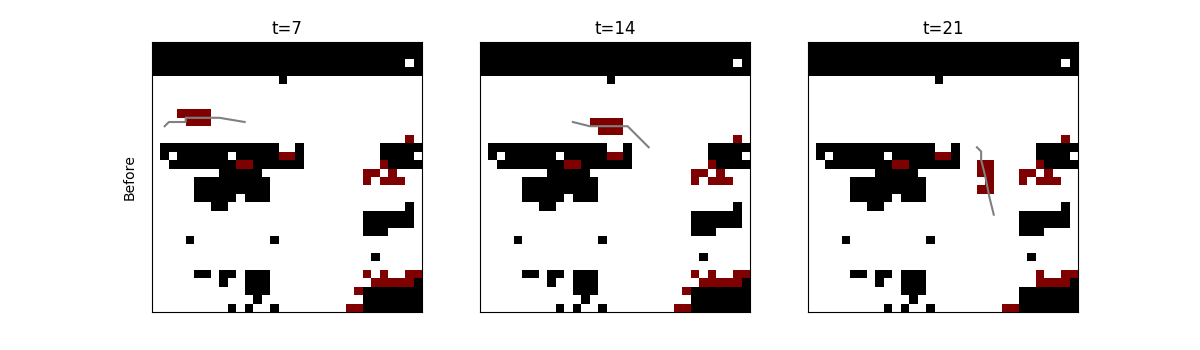
\includegraphics[width=\textwidth]{figures/before.png} \\
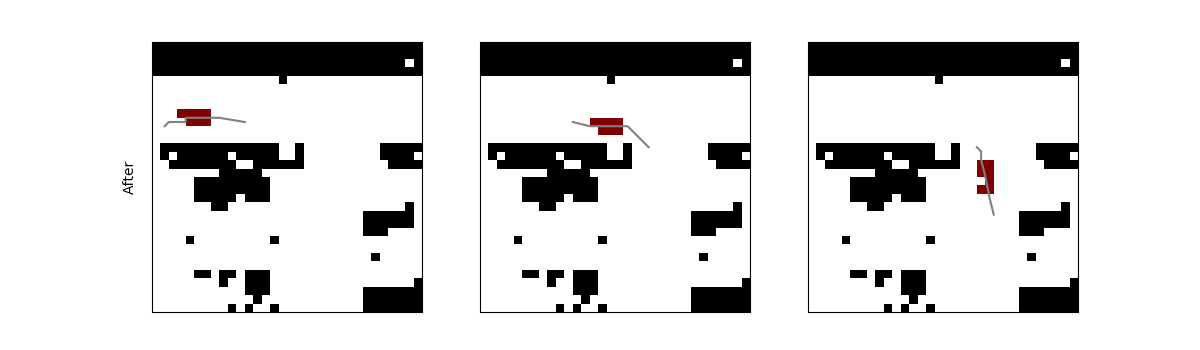
\includegraphics[width=\textwidth]{figures/after.png}
\caption[One example of preprocessing of real data.]{One example of preprocessing of real data. Black cells are from the static map. Red and white cells represent \textit{occupied} and \textit{not occupied} respectively. A person is identified by a blob of occupied cells and the gray line indicates the trajectory. \textbf{Upper}: The real data recorded by laser scanners. \textbf{Lower}: The corresponding data after preprocessing. One can see that, the noisy occupancies are removed without affecting the dynamics of human motion.} 
\label{fig:preprocessing}
\end{figure}

 \begin{figure}[H]
\centering
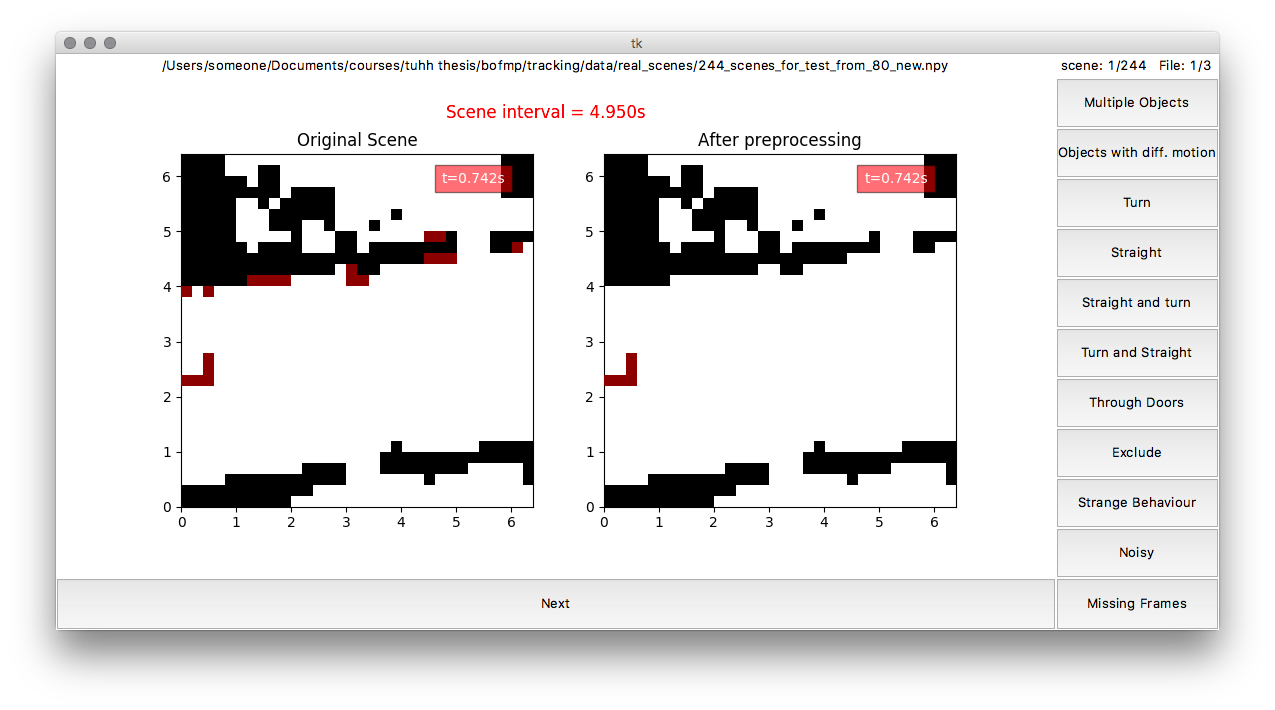
\includegraphics[width=.9\textwidth]{figures/application_1.png}
\caption[Application used for labeling scenes.]{Application used for labeling scenes. User can define their own classes, which are shown as buttons on the right. On the left, both the original scene and preprocessed scene are displayed as animations. User can continue labeling by clicking ``Next'' button.} 
\label{fig:application}
\end{figure}

\section{Implementation of BOFMP} \label{sec:BOFMP_implementation}

\subsection{Extension of Network Output} \label{sec:mm_ext}

As described in Section \ref{sec:traj_sim}, the motion pattern extracted from network output considers max speed of 1 $cell/timestep$. However, since human does not always walk in a constant speed, we need to adapt our motion model to higher speeds. This is done by applying Gaussian blur in acceleration space. For now, we omit the cell index $c$, and the motion pattern from network output is represented as:
\begin{equation}
P_{NN}(v^{ex}=(v^{ex}_x, v^{ex}_y)|v^{en}=(v^{en}_x, v^{en}_y)) \label{eq:mm_1}
\end{equation}

where $v^{ex}_x, v^{ex}_y,v^{en}_x, v^{en}_y \in [-1, 1] \cap \mathbb{Z}$. We define the \textit{extent} as the number of values that velocity can take in either $x$ or $y$ axis. Due to its symmetry, the max speed for extent $e$ is $\lfloor \frac{e}{2} \rfloor$ cell/step. Therefore, $P_{NN}$ has an extent $e_{n}$ of 3 and dimension of $3 \times 3 \times 3 \times 3$. 

Let us assume that we want motion model for extent $e_w$. This is achieved by firstly padding $P_{NN}$ to dimension $e_w \times e_w \times e_w \times e_w$ with zeros, s.t., $v^{ex}_x, v^{ex}_y,v^{en}_x, v^{en}_y \in [-\lfloor \frac{e_w}{2} \rfloor, \lfloor \frac{e_w}{2} \rfloor] \cap \mathbb{Z}$ . Then we can calculate the probabilities for acceleration conditioned on entering velocity:
\begin{equation}
P_{NN}(a|v^{en}) = P_{NN}(v^{ex}=v^{en}+a|v^{en}) \label{eq:mm_2}
\end{equation}

With a 4-dimensional Gaussian kernel $K(a, b) \sim \mathcal{N}((a,b), \Sigma)$, we have:
\begin{equation}
P(a|v^{en}) = \sum_{\hat{a}, \hat{v}^{en}}P_{NN}(\hat{a}|\hat{v}^{en})\times K(\hat{a}, \hat{v}^{en}) \label{eq:mm_3} 
\end{equation}

Finally we get motion pattern $P(v^{ex}|v^{en})$ by restoring to velocity space and normalization:
\begin{align}
\hat{P}(v^{ex}|v^{en}) &= P(a=v^{ex}-v^{en}|v^{en}) \\
P(v^{ex}|v^{en}) &= \frac{\hat{P}(v^{ex}|v^{en})}{\sum_{v^{ex}}\hat{P}(v^{ex}|v^{en})} \label{eq:mm_4}
\end{align}

One example is shown in Figure \ref{fig:mm_ext}. As can be seen from the figure, the original motion pattern $P_{NN}(v^{ex}|v^{en}$ has max speed of 1 $cell/step$, while for the extend one $P(v^{ex}|v^{en})$ the max speed is 2 $cell/step$. From the extended motion pattern $P(v^{ex}|v^{en})$, one can see that only the directions of velocity change but not the speed. This implies that even if a person changes his or her walking direction, the walking speed is normally not changed.

\begin{figure}[hp]
\begin{tabular}{cc}
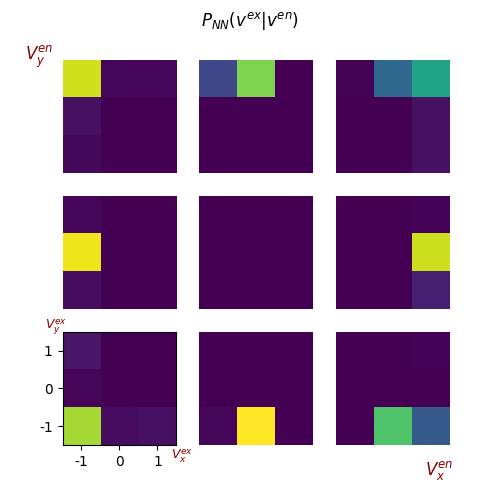
\includegraphics[width=0.5\textwidth]{figures/mm_ext_1.png}
&
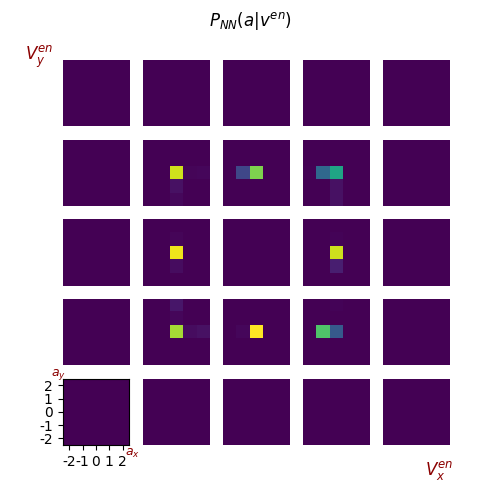
\includegraphics[width=0.5\textwidth]{figures/mm_ext_2.png} \\
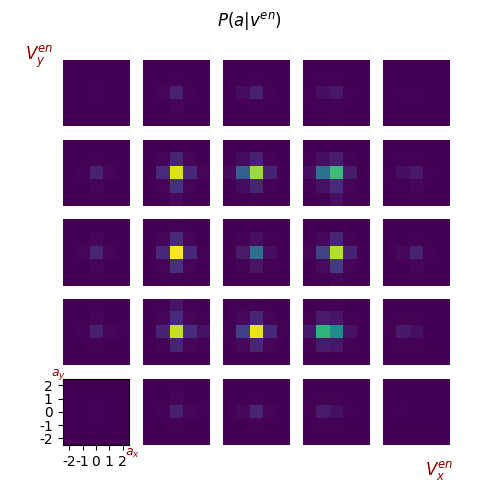
\includegraphics[width=0.5\textwidth]{figures/mm_ext_3.png}
&
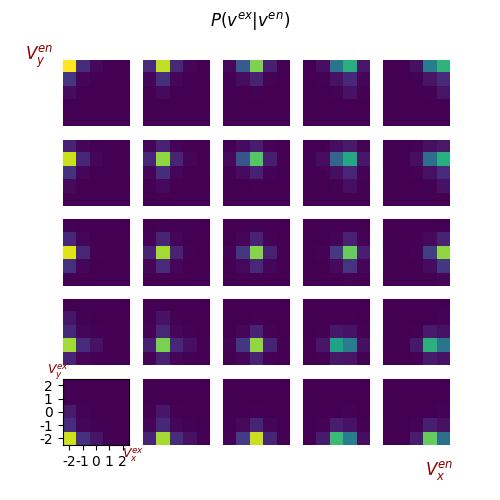
\includegraphics[width=0.5\textwidth]{figures/mm_ext_4.png}
\end{tabular} 
\caption[One example of extending motion pattern probabilities from network output to higher extent.]{One example of extending motion pattern from network output to higher extent. The definitions of these quantities shown in figure are explained in Equation \ref{eq:mm_1} $\sim$ \ref{eq:mm_4}. The original motion pattern $P_{NN}(v^{ex}|v^{en})$ has max speed of 1 $cell/step$, while for the extend one $P(v^{ex}|v^{en})$ the max speed is 2 $cell/step$. This is achieved by applying Gaussian blurring in acceleration space. From the extended motion pattern $P(v^{ex}|v^{en})$, one can see that only the directions of velocity change but not the speed (in fact, with a small probability to accelerate or decelerate). This implies that even if a person changes his or her walking direction, the walking speed is normally not changed.} 
\label{fig:mm_ext}
\end{figure}

\subsection{Workflow of BOFMP}

Before introducing the workflow of our method, some parameters that used to initialize BOFMP must be clarified:

\begin{my_enumerate}
\item \textbf{extent \( e\)}. As introduce in \ref{sec:mm_ext}, extent is defined as the number of values that velocity can take in either $x$ or $y$ axis.	For example, if extent is 7, the velocities on both $x$ and $y$ axis must be integers within range  \( [-3, 3] \). The extent determines the maximum speed speed our algorithm concerns. 
\item \textbf{variance \( \delta^2\)}. For BOFUM, this parameter refers to the variance of the Gaussian distributed acceleration noise in Equation \ref{eq:adding_noise}. For BOFMP, it is the variance of the Gaussian kernel used for blurring in Equation \ref{eq:mm_3}. In both cases, this parameter reflects the algorithm's belief on how likely an object accelerates or decelerate.
\item \textbf{omega \( \Omega \)}. In the correction step of BOF filters, measurements from sensors are taken into account for estimating the posterior probability. Since sensor could be noisy, this parameter determines how much does the filter trusts the measurements. The sensor used for in our tracking application is laser scanners, which is rather physically reliable and therefore has a low \( \Omega \) value.
\end{my_enumerate}

A trained CNN model that used for extracting motion pattern from static map must be available. With the above parameters being defined and the CNN model being ready, the BOFMP filter can be applied. Firstly, feed the static map to the network so that $P_{NN}(V^{ex}|V^{en})$ is retrieved. It is then extended to the desired extent $e$ to get motion pattern $P(V^{ex}|V^{en})$. Before the filtering starts, the occupancy and velocity probabilities are initialized uniformly, i.e. for $c=1:N$,
\begin{gather}
P(O_c = occ) = P(O_c = nocc)=0.5 \\
P(V_c=v) = \frac{1}{e^2}
\end{gather}

 After initialization, the actual tracking can start by recursively executing tracking step. A tracking step is composed of two steps: \textit{prediction} and \textit{estimation}. In prediction step, a prior distribution of the state of cells is derived. In estimation step, a posterior distribution is calculated by multiplying the prior distribution with a conditional probability distribution that represents correction based on incoming measurements. However, the measurement gives information about only whether a cell is occupied or not at each time step. In order to make proper predictions for the next time step, the filter has to infer velocities for each cell. To get some intuitions, Figure \ref{fig:correction} shows an example of tracking step. The complete workflow is illustrated in Figure \ref{fig:fitering_workflow}.

\begin{figure}[H]
  \centering
    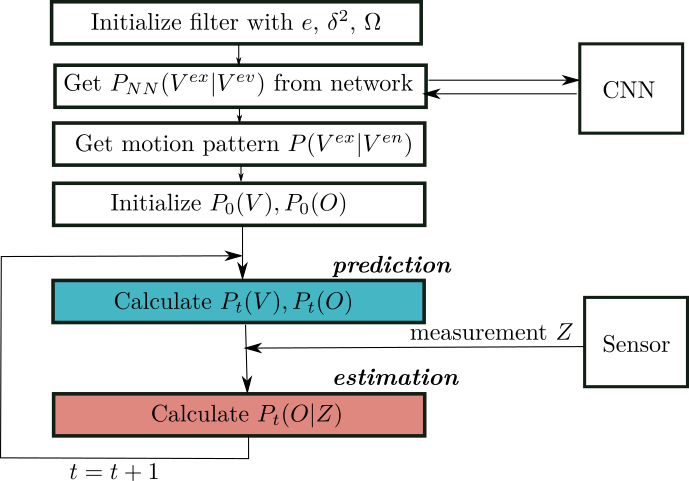
\includegraphics[width=.7\textwidth]{figures/filtering_workflow.png}
    \caption[Workflow of BOFMP filter.]{Workflow of BOFMP filter. The parameters of the filter have to be defined firstly. The motion pattern probabilities are obtained from the outputs of a pre-trained CNN. The state of cells are initialized with uniform distributions and then recursively updated by prediction and estimation step. Measurements from sensor are used for estimation.}
    \label{fig:fitering_workflow}
\end{figure}

\begin{figure}[ht]
  \centering
    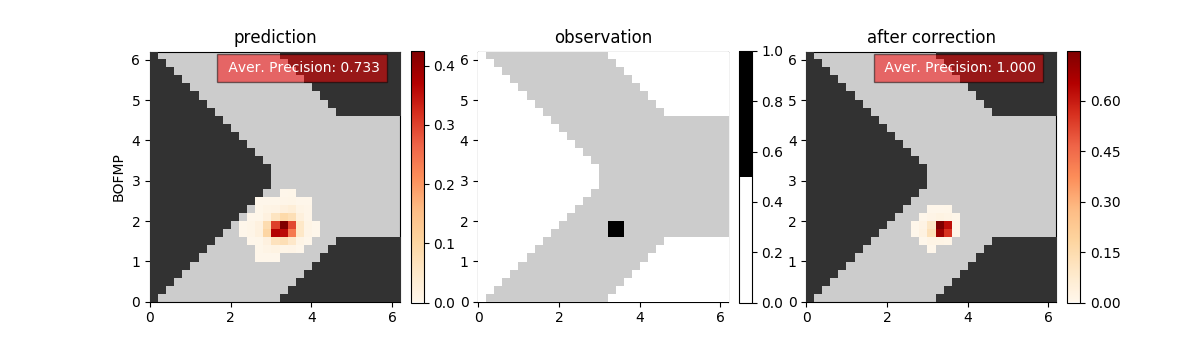
\includegraphics[width=\textwidth]{figures/correction_step.png}
    \caption[One filtering step of BOFMP filter.]{One filtering step of BOFMP filter. At last time step, the person goes from up to down. Based on motion pattern, BOFMP predicts that there are possibilities that this person will turn to left-down and keep going downwards. After measurement shows that this person still goes downwards, BOFMP corrects its predictions and attenuates probabilities of turning left-down. Since the measurement adds additional information for BOFMP to make better predictions, the average precision increases after correction step.}
    \label{fig:correction}
\end{figure}

\subsection{Code Structure}

The functionalities of the code concern mainly three parts:
\begin{my_enumerate}
\item \textbf{Tracking filters}. Both BOFMP and the baseline BOFUM filters are implemented. Besides, based on the data used, i.e., either simulated data or real data, the implementation has to be different. 
\item \textbf{Visualization of tracking}. To have a better idea about how tracking performs, visualization of tracking for each time step is necessary. We implemented two ways of visualization. One is to show tracking step by step as prediction and correction with static plots. The other shows the tracking process with animation. 
\item \textbf{Evaluation on tracking performance}. In order to compare our method with its baseline, evaluation on tracking performance is necessary. The metric used for evaluation is described in Section \ref{sec:metrics}.
\end{my_enumerate}

We follow an object-oriented programming paradigm. By defining classes and subclasses, this facilitates code reuse and better structure of the code. Figure \ref{fig:classes} shows the main classes defined in the code. They are grouped based on their functionalities. 

\begin{figure}[hp]
  \centering
    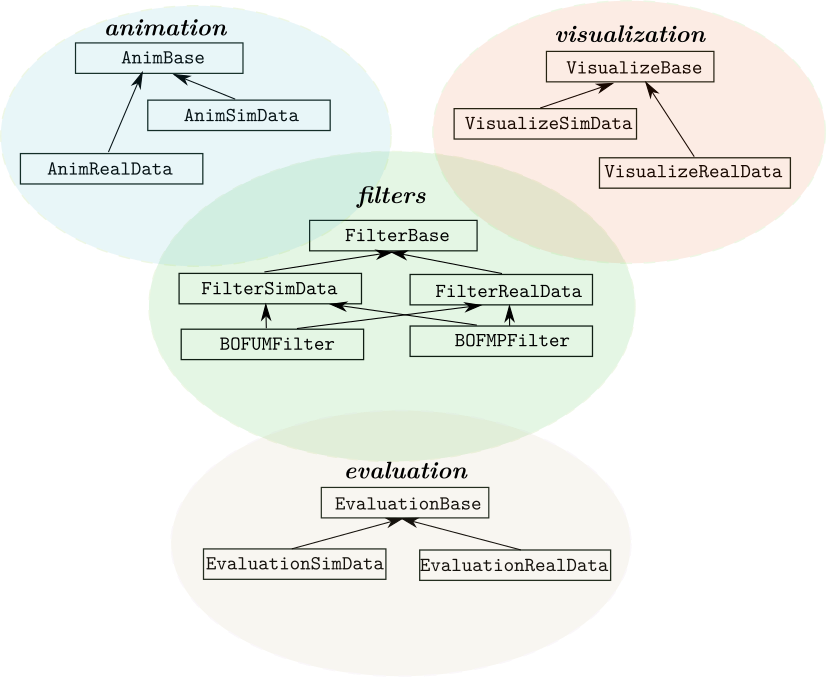
\includegraphics[width=\textwidth]{figures/classes.png}
    \caption[Classes defined in the code.]{Classes defined in the code. Classes are grouped according to their functionalities. The ``filters'' is shown in the center since it is used by other classes. The arrows show class inheritance. For example, \texttt{ClassA} $\rightarrow$ \texttt{ClassB} indicates that \texttt{ClassA} is inherited from \texttt{ClassB}. }
    \label{fig:classes}
\end{figure}



\cleardoublepage
%!TEX root = ThesisLKN.tex
\chapter{Results and Discussions} \label{chapter:5}


\section{Metrics}

\subsection{Metrics for Neural Network}

\subsection{Metrics for Tracking}

\section{Training of Neural Network}

After the data is collected as described in Section \ref{sec:traj_sim}, we split them into training, validation and test set. The training and validation set are sampled from seven full maps, and test set is sampled from a separate map. The number of samples we generated are summarized in Table \ref{table:nos}. 

Figure \ref{fig:trajs} shows one example of map window as network input and its ground truth. On the left, a cell is labeled with red color, and the sampled trajectories that go through this cell are displayed. On the right, it shows a visualization of the ground truth \( P_c(V^{ex} | V^{en}) \) for that red cell. The axes show velocities on \( x, y\) directions. Since we assume a person has maximum speed of 1 $cell/timestep$, the velocities must be in range $[-1,1]. $Outer axes represent entering direction \( V^{en} \), and inner represents exit velocity \( V^{ex} \). One can see that \( P(V^{ex}=DL | V^{en}=DL) = 0.13 \) and \( P(V^{ex}=D | V^{en}=DL) = 0.87 \) \footnote{DL represents going down-left, and its corresponding velocity is (-1, -1). D represents going down, and its velocity is (0, -1).}. This indicates that if a person reaches the red cell by taking direction down-left (i.e., coming from upper-right neighboring cell), it is very likely that he or she will change to going down for the next time step. This proves that our way of modeling motion pattern captures human motion dynamics.

\begin{table}[t]
\centering
  \begin{tabular}{c|ccc}
    \hline
     & training & validation & test \\ \hline
    number of samples & 27,119 & 4,785 & 3,760\\
    \hline
  \end{tabular}
\caption{Number of samples in training, validation and test set.}
\label{table:nos}
\end{table}

\begin{figure}[H]
\begin{tabular}{ll}
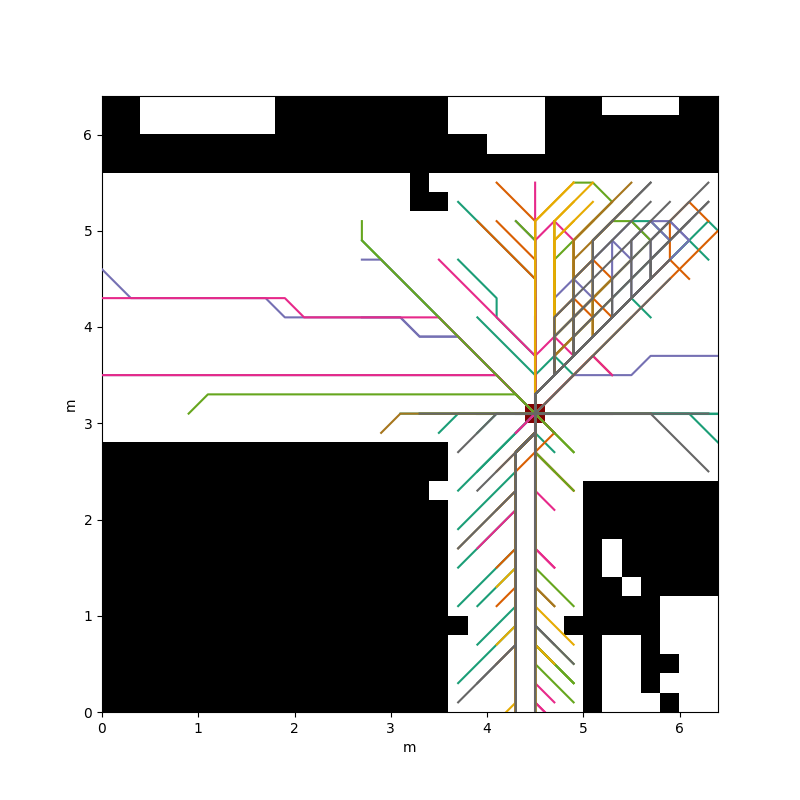
\includegraphics[width=0.48\textwidth]{figures/trajs_through_cell.png}
&
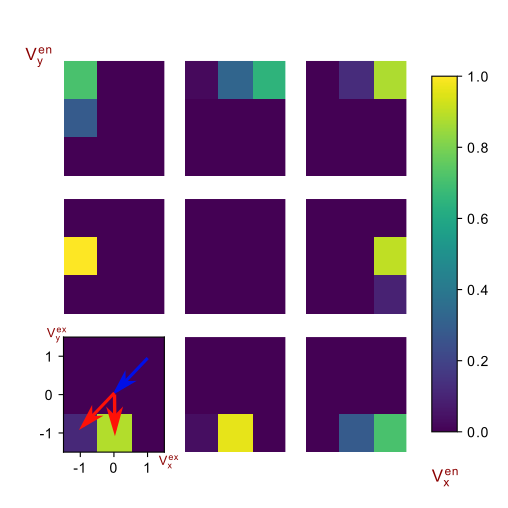
\includegraphics[width=0.48\textwidth]{figures/probs_on_that_cell_2.png}
\end{tabular}
\caption[one example of map window as network input and its ground truth]{one example of map window as network input and its ground truth \textbf{Left}: The map window has size of \( 32 \times 32 \) cells, with resolution of \( 0.2m/cell\). It also shows trajectories that goes through the red cell. \textbf{Right}: Visualization of conditional probability \( P_c(V^{ex} | V^{en}) \) for the red cell on left map. It can be seen that if a person reaches that cell by taking down-left direction, it is very like that he or she will change direction to going down.}. 
\label{fig:trajs}
\end{figure}

\section{Evaluation of Tracking Performance}

\subsection{Overview of Datasets}

\textbf{Simulated Dataset}

\textbf{Real Dataset}

\subsection{Tracking on Simulated Data}

\subsection{Tracking on Real Data}

\section{Applications}

\textbf{Dynamic Analysis}

\textbf{Get occupancy map}


 

\cleardoublepage
%!TEX root = ThesisLKN.tex
\chapter{Conclusions and Outlooks} \label{chapter:6}

1. train on simulation, but works on real data.

contribution:
implement BOFUM with python

\section{End to End Training}

\section{Future Work}
%Recurrent Tracking Network with Motion Model

\cleardoublepage
%!TEX root = ThesisLKN.tex
\chapter{Summary of Results}

This thesis focuses on human tracking in indoor environments, such as offices and factories. In those environments, since there exists static obstacles, e.g., walls, tables, the tracking algorithm needs to differentiate between static obstacles and moving humans. One general tracking algorithm from literature is called as \textit{Bayesian Occupancy Filter}(BOF). It represents the environment as a grid map, and it predicts the occupancy probability of each cell for every time step. An improved version of BOF is \textit{Bayesian Occupancy Filter Using Map knowledge}(BOFUM). As its name indicates, it utilizes prior map knowledge about how likely a tracking object might be on different locations on a given map. 

\begin{figure}[ht]
  \centering
    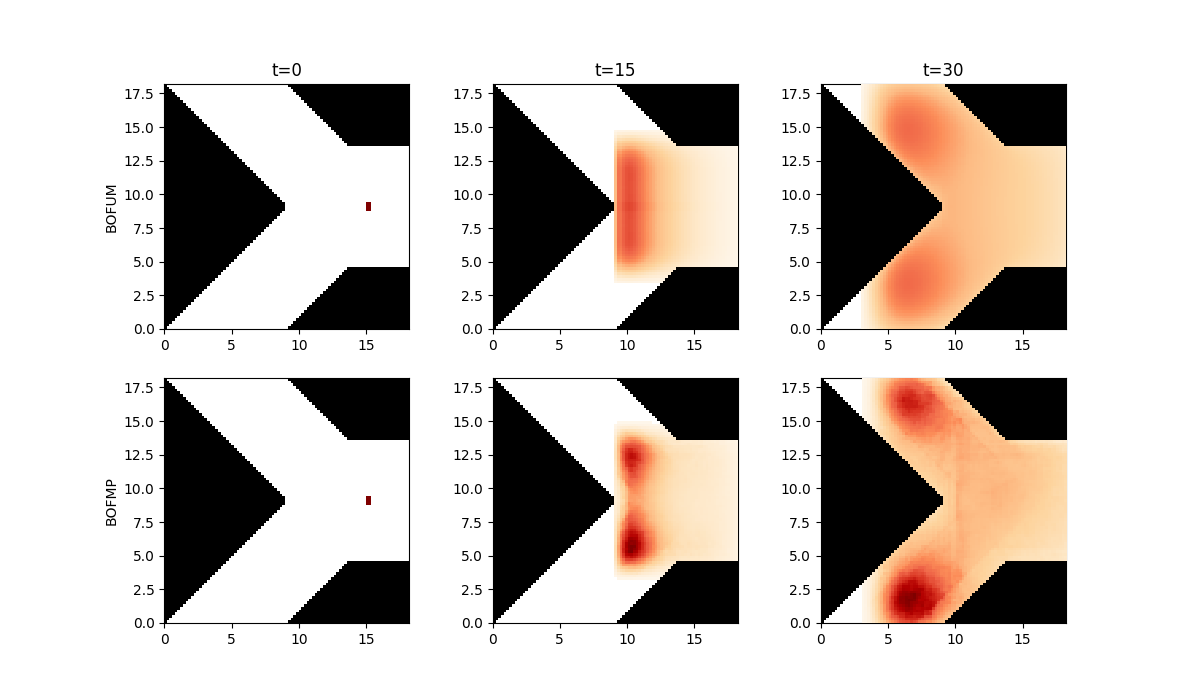
\includegraphics[width=\textwidth]{figures/idea.png}
    \caption{Occupancy predictions for BOFUM and our proposed BOFMP after several time steps. The map shows a T-section. At $t=0$, a person is shown as a red rectangle and with initial velocity towards left. At $t=15$, the person encounters intersection. BOFUM has no information about human motion pattern, and continues to propagate occupancy towards left. Our BOFMP knows that humans are likely to turn to either upper or lower corridors. At $t=30$, since occupancies going left vanish due to the wall, BOFUM predicts occupancies in corridors, but they are biased towards walls on the left. Our BOFMP predicts more occupancies in the middle of corridors, since it knows humans are more likely to walk in the middle.}
    \label{fig:idea}
\end{figure}

Human trajectories in indoor environment follow some motion patterns. For example, when there is corridor, humans tend to walk in the middle of the corridor, instead of walking besides the walls. To incoporate this human motion into tracking algorithm, we proposed \textit{Bayesian Occupancy Filte Using Motion Pattern}(BOFMP). The idea is shown in Figure \ref{fig:idea}.

The main contributions of this thesis work are summarized as following:

\begin{my_enumerate}
\item Neural Network Training.
\item Human Trajectory Simulation.
\item Object Tracking using Bayesian Occupancy Filter
\item Comparision between BOFUM and BOFMP
\end{my_enumerate}

\section{ Neural Network Training}  To capture  human motion patterns, we trained neural networks to learn how a walking person changes directions at different locations on a given map. Mathmatically, there are two ways to represent the motion pattern, either using conditional probability or joint probability. For the former one, given a grid map as input, the network learns for each given grid cell \( c \) on the map, the probabilities of next possible velocity \( V \) conditioned on last velocity \( V^- \):

\[ P_c\{V | V^-\} \] 

Alternatively, the network can also learn the joint probability:

\[ P_c\{V , V^-\} \]

Theoretically, it is always better to have joint probability, since conditional probability can be caculated from joint probability by marginalization and Baye's rule. However, due to reasons explained in Section \ref{section:hms}, we are not able to get accurate joint probabilities as ground truth. Therefore, the network is trained to learn \( P_c\{V | V^-\} \). 

\begin{figure}[ht]
  \centering
    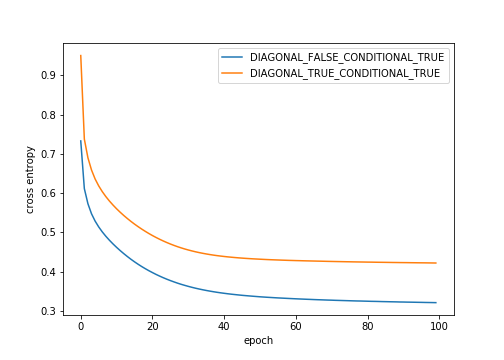
\includegraphics[width=.7\textwidth]{figures/trainning_history.png}
    \caption{Cross entropy loss for trainning networks. We trained networks to learn conditional probabilities \( P_c\{V | V^-\} \). The green line shows trainning dynamics using data generated with directions "left, right, up and down". The yellow line also takes diagonal directions into account, which has 8 directions in total. Naturally, since more directions implies higher complexity, the overall loss for yellow line is higher than green line.}
    \label{fig:trainning}
\end{figure}

The network consists of 31 convolutional layers. It has both down-sampling path for extracting high-level features and up-sampling path for recovering full resolution. The network is trained with mini-batches of size of 128, and  is optimized with Adam optimizer. The training runs for 100 epoches, with early stopping patience of 15 epoches. Figure \ref{fig:trainning} shows the cross entropy loss during training.

\section{Human Trajectory Simulation} \label{section:hms}

To acquire enough amount of data for trainning our netwrok is expensive, especially when we have to consider all possible motion changes for every cell in a grid map. For non-diagonal directions, there are \( 4\times4=16\) possible motion changes. For diagonal directions, it goes up to \( 8\times8=64\). To get statistically sound motion pattern probabilities, it requires to record human trajectories on many different maps over a long period of time. However, due to practical reasons, we are not able to get that much real data. Instead, we simulate human trajectories with A-star algorithm from 6 real world maps with a total free space area of ca. \( 6.6\times10^3 \, m^2 \). For each cell on the map, we try to sample 5 trajectories starting from that cell. With those trajectories, we can caculate motion pattern probabilities. Then we take random crops of size \( 32 \times 32 \) cells from the real world maps as network inputs, and their corresponding probabilities as outputs. 

% \figtwo{trajs\_through\_cell, trajs\_through\_cell, caption, trajs, htbp }

\begin{figure}[t]
\begin{tabular}{ll}
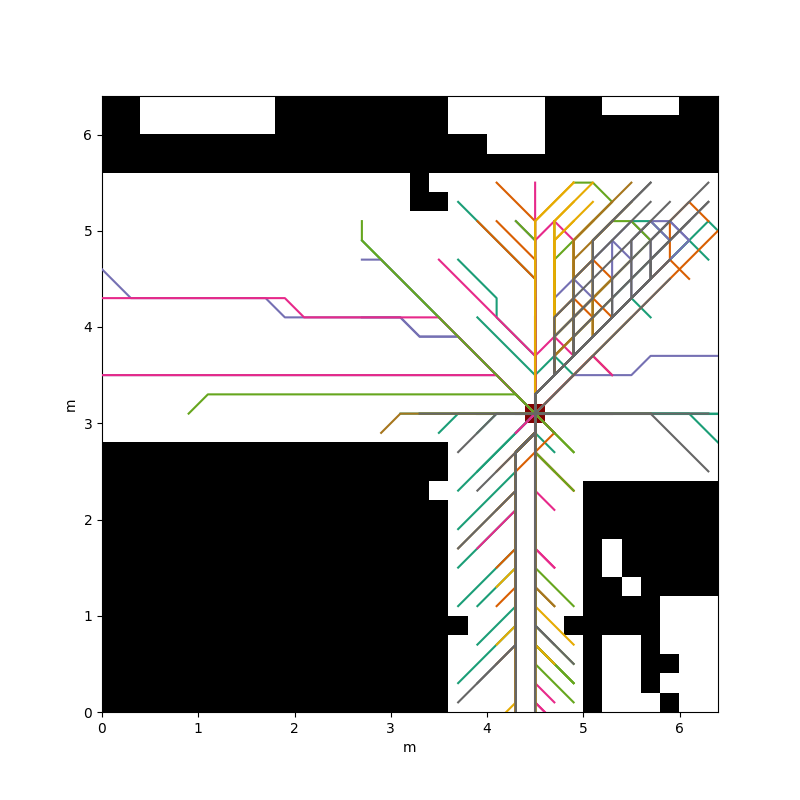
\includegraphics[width=0.48\textwidth]{figures/trajs_through_cell.png}
&
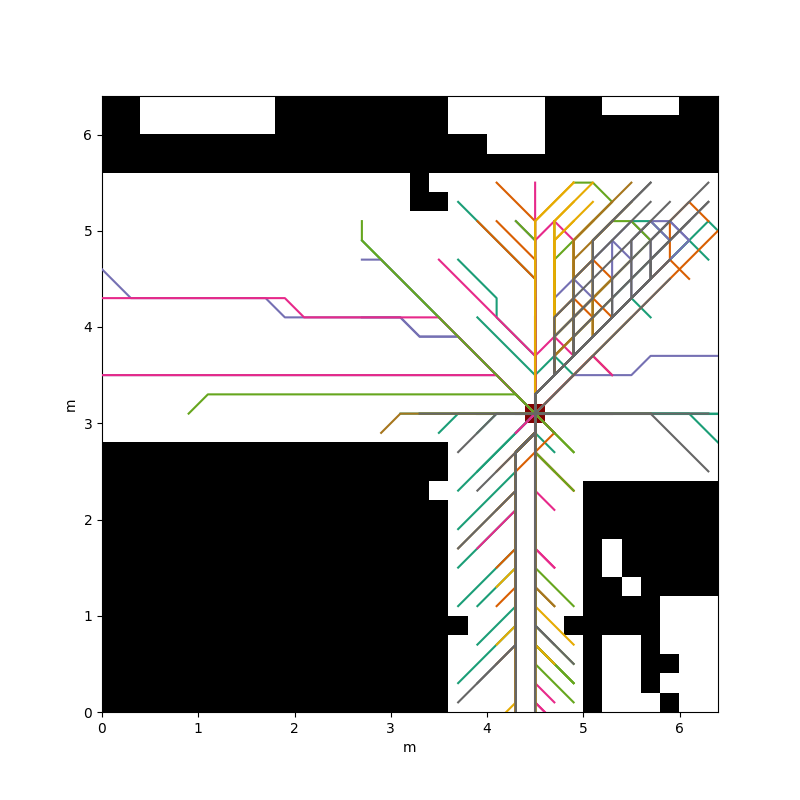
\includegraphics[width=0.48\textwidth]{figures/trajs_through_cell.png}
\end{tabular}
\caption{\textbf{Left}: One example map crop as netwrok input. The map has size of \( 32 \times 32 \) cells, with resolution of \( 0.2m/cell\). It also shows trajectories that goes through the red cell. \textbf{Right}: Visualization of conditional probability \( P\{V | V^-\} \) for the red cell on left map. The axis shows velocities on \( x, y\) directions. Outter axes represent last velocity \( V^- \), and inner represent next velocity \( V \). One can see that \( P\{V=(-1, -1) | V^-=(-1, -1)\} = 0.21 \) and \( P\{V=(0, -1) | V^-=(-1, -1)\} = 0.79 \). This indicates that if a person reaches the red cell from upper right, it is very likely he will go downwards. }. 
\label{fig:trajs}
\end{figure}

Figure \ref{fig:trajs} shows one example of network input and the ground truth for one cell on the map. The number of samples we generated are summarized as follows:

\begin{center}
  \begin{tabular}{c|ccc}
    \hline
     & trainning & validation & test \\ \hline
    number of samples & 27,119 & 4,785 & 3,760\\
    \hline
  \end{tabular}
\end{center}

\section{Object Tracking using Bayesian Occupancy Filter}

Generally, Bayesian filter works in a recursive way and the filtering process can be decomposed into two stages: \textbf{prediction} and \textbf{correction}. For each time step, it firstly predicts the next state. After prediciton, when the new measurement is obtained, it corrects its prediction based on measurement. For Bayesian occupancy filter used in tracking applications, the state of world is represented by, for each cell on the grid map, the probabilities of cell's velocities and occupancy. However, the measurement gives information about only whether a cell is occupied or not at each time step. In order to make predicitions for the next time step, the filter has to infer velocities of each cell based on past occupancy information from measurements. Figure \ref{fig:correction} shows how BOFMP filter updates at one time step.


\begin{figure}[ht]
  \centering
    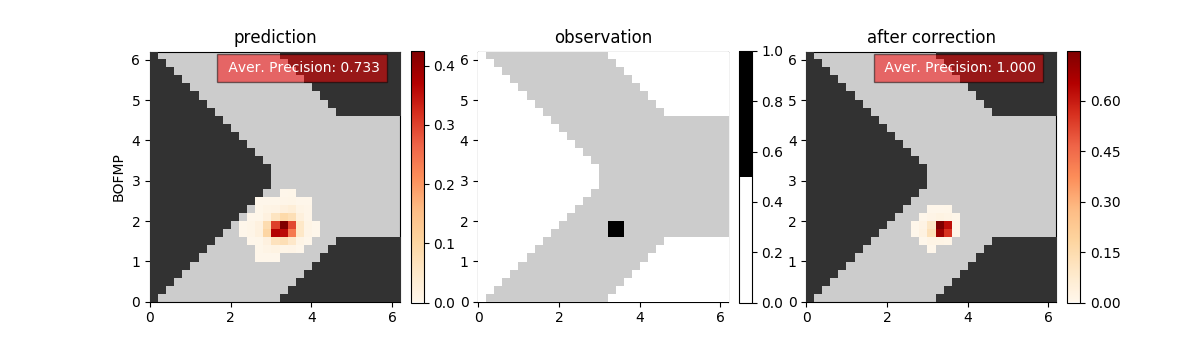
\includegraphics[width=\textwidth]{figures/correction_step.png}
    \caption{One filtering step of BOFMP filter. At last time step, the tracking object goes from up to down. Based on motion pattern, BOFMP predicts that there are possibilities that this object will trun to left-down and keep going downwards. After measurement shows that this obejct still goes downwards, BOFMP corrects its predictions and attenuates probabilities of turning left-down. Since the measurement adds additional information for BOFMP to make better predictions, the average precision increases after correction step.}
    \label{fig:correction}
\end{figure}

\section{Comparision between BOFUM and BOFMP}

To compare the performance of BOFUM and BOFMP, we consider two scenarios:

\begin{my_enumerate}
\item \textbf{tracking}. Measurements are given at each time step, and we evaluate consistency between occupancy predicton and the ground truth at every time step before a certain time point \( t \) .
\item \textbf{future prediction}. From time point \( t \) on, the measurement is no longer given. Then we evaluate occupancy predictions with ground truth for the next \( n \) time steps.
\end{my_enumerate}

The parameters of a BOF filter are:
\begin{my_enumerate}
\item \textbf{extent \( e\)}. It determines the maximum velocity of a cell. For example, if extent is 7, the velocities are in range  \( [-3, 3] \) cells/time step on both \( x \) and \( y \) axis. Since our neural network only models velocities within \( [-1, 1]\), we need firstly extend it to higher velocities. The details on how we do this will be explained in the thesis. 
\item \textbf{noise variance \( \delta^2\)}. Both BOFUM and BOFMP assume the tracking object has a constant velocity, with a Gaussian distributed acceleration noise. This parameter determines how likely an object accelerates or decelerate.
\item \textbf{omega \( \Omega \)}. In the correction step of BOF filters, measurments from sensors are incorporated into filter's prediction. Since sensor could be noisy, this parameter determines how much do we trust our measurements. The sensor used for our tracking application is laser rangefinder, which is rather physically reliable and therefore has a low \( \Omega \) value.
\end{my_enumerate}

The possible metrics that could be used for measuring the consistency between occupancy predicition and ground truth are: \textit{cross entropy}, \textit{f1 score} and \textit{average precision}.  We choose average precision as our metric and the reasons will be detailed in the thesis. To prove that our method is able to make predictions according to human motion pattern, we tune the parameters based on filter's performance for future predictions. For both filters, we randomly sample 100 sets of parameters from parameter ranges listed in Table \ref{table:param_range}, evaluate on tracking cases with time steps of 16 and caculate average precision for every time step over all tracking cases. Note that value range of noise variance $\delta^2$ for real data is higher than for simulated data. This is because in real data, there are higher uncertainties with human motion and sensor failures. The measurement is lost at time step \( t=9\), and we select the best set of parameters based on the average of average precisions for the next \( 8 \) time steps. 

\begin{table}[H]
\centering
  \begin{tabular}{c|c|c}
    \hline
     &   value range for simulated data & value range for real data \\ \hline
    \( e \) & \( \{3, 5, 7\} \) &  \( \{3, 5, 7\} \)\\
    \(  \delta^2\) & \( [0.1, 0.6]\) & \( [0.2, 0.7]\) \\   
   \( \Omega \) & \( [0.01, 0.2] \) & \( [0.01, 0.2] \)\\
   \hline
 \end{tabular}
\label{table:param_range}
\caption{Parameter ranges for BOF filters.}
\end{table}

\subsection{On simulated data}

We generated 500 tracking cases as validation set for tuning filter parameters and 500 tracking cases for test set. Validation and test cases are generated from different maps, and on each map, there are either one or two walking humans. We firstly tuned the parameters on validation set for BOFUM and BOFMP individually. Then we apply both filters with their best parameters on test set. The best set of parameters and its corresponding average precision from \( t=9 \) to \( t=16 \) on test data are listed in Table \ref{table:best_param_simulated}. Figure \ref{fig:simulated_test_data} shows mean of average precision over 500 test cases for each time step.

\begin{table}[H]
\centering  
\begin{tabularx}{\textwidth}{c|c|c|c|c|c}
    \hline
    & $ e $ & $ \delta^2 $ & $ \Omega $ & average precision for $t=8:16 $ & mean\\ \hline
    BOFUM & 7 & 0.556 & 0.0164 &  0.767  0.599  0.500    0.416  0.349  0.279  0.232  0.192 & 0.417 \\
    BOFMP & 7 & 0.373 & 0.0353 & 0.785  0.637  0.552  0.479  0.416  0.358  0.311  0.252 & 0.474 \\
   \hline
  \end{tabularx}
\label{table:best_param_simulated}
\caption{Best parameters for BOFUM and BOFMP on simulated data.}
\end{table}


\begin{figure}[ht]
  \centering
    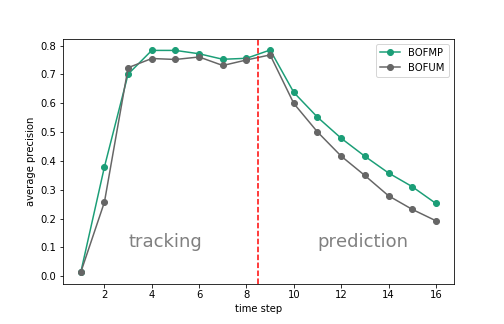
\includegraphics[width=.8\textwidth]{figures/test_on_simulated_data.png}
    \caption{Evaluation results on test data. The average precision for both filters start with values close to zero. Since we highly trust our measurments (low $\Omega$), both filters are able to successfully track the objects within 3 time steps. The fact that average precision keeps a high vaule from $t=3$ to $t=8$ indicates that both filters can predict very well for the next immediate time step. Starting from $t=9$ (see the red dash line), measurements are no longer given. The prediction is still accurate for the next time step ($t=9$), but decreases progressively over time.  This is expected, since without measurements, the state of world becomes more and more uncertain. Even though, we can see that our BOFMP have a higher average precision value than BOFUM at almost every time step, which indicates the improvements of our method in both tracking and future predicition stages.}
    \label{fig:simulated_test_data}
\end{figure}

Figure \ref{fig:tracking_simulated_data} shows how BOFUM and BOFMP perform tracking on one case from test data. In this example, a person is walking from the lower door towards upper door. The grey curve on the map shows the trajectory of the person. At $t=8$, the person walks with upwards velocity of 1 cell/time step. Both algorithms track the person very well with average precision of $1.0$. At $t=9$, the measurement is lost and future prediction stage of tracking starts. At $t=10$, BOFUM predicts that the person will still goes upwards, with a low possibility going other directions. However, since BOFMP knows there is a door above, it predicts that the person is also very likely going to that door, and therefore turns to upper left. At later time steps, BOFMP continues to predict occupancy probabilities towards upper door as well as other possible directions (i.e., door on the left and empty space on the right). On the contrary, BOFUM still propagates most occupancies upwards. At $t=16$, since the object accelerates to higher velocity, most of occupancy predictions of BOFMP are left behind the tracking object.
\begin{figure}[ht]
  \centering
    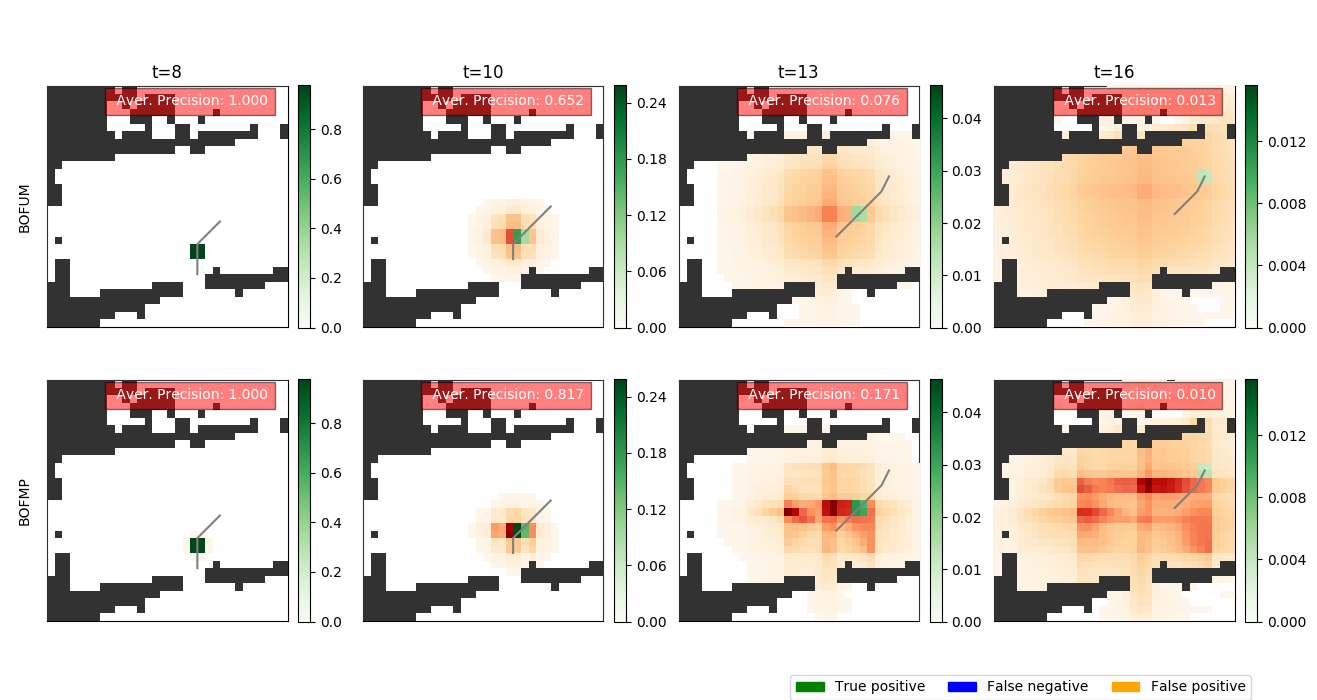
\includegraphics[width=\textwidth]{figures/tracking_sample_for_simulated_data.png}
    \caption{One example of tracking case from test data.}
    \label{fig:tracking_simulated_data}
\end{figure}

\subsection{On real data}

Although our neural network are trained on simulated human trajectories, we expect that our method also outperforms BOFUM on real tracking cases. We recorded human trajectories on two different ground plans by a laser rangefinder mounted on a robot. After processing raw laser data, we get 500 tracking cases for validation from one of the ground plans and 244 for test from the other. 



\textbf{Spatial blurring of motion probabilities}

The simulated trajectories do not always reflect real human's motion patterns. This is because, as shown in Figure \ref{fig:blur_idea}, humans are more flexible to decide when to make turns. 

\begin{figure}[ht]
  \centering
   \captionsetup{width=\linewidth}
    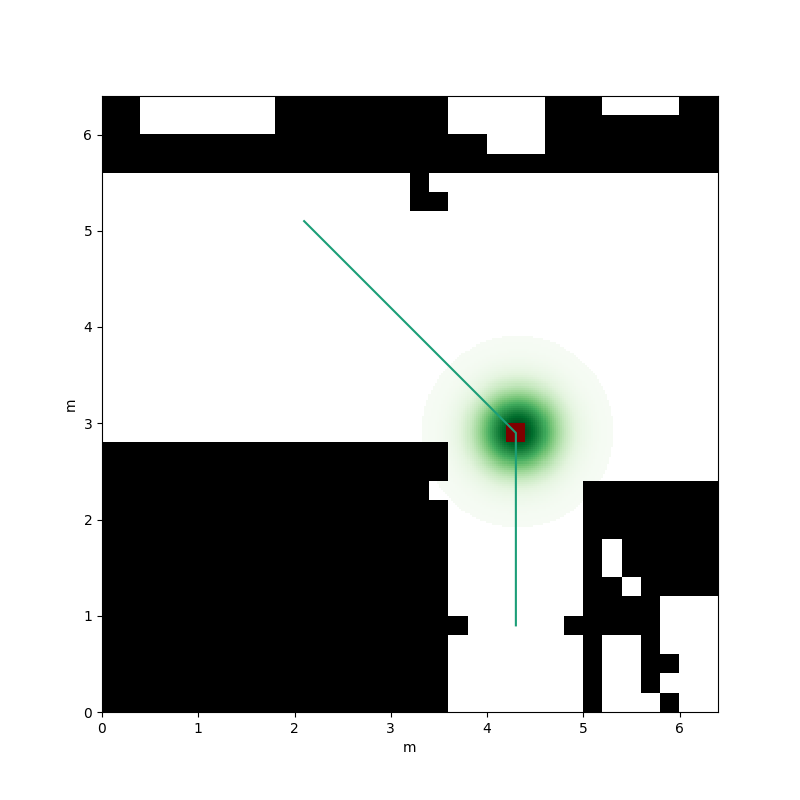
\includegraphics[width=.6\textwidth]{figures/blur_idea.png}
    \caption{A turn on simulated human trajectory. In order to reach the goal location in upper left corner, the simulated trajectory shows that a person will make a turn from going up to going up-left at location indicated by the red square. However, in real scenarios, a person is more flexible in deciding where to make that turn and he might turn at any location in the green area.}
    \label{fig:blur_idea}
\end{figure}

Therefore, to better adapt to real data, we introduce a techinique that blurs the motion probabilities  \( P_c\{V | V^-=v\} \) of a cell $c$ spatially into its neighbors if a \textit{turn} is detected. A \textit{turn} on cell $c$ for velocity $v^-$ is defined as:

\[ 
turn_c(v^-) = 
\begin{cases}
    True , & \text{if} \quad \argmax_v (P_c\{V=v | V^-=v^-\}) \, != \, v^- \\
    False,              & \text{otherwise}
\end{cases}
 \]


For each turn detected from motion pattern, we apply Gaussian blur spaitally to its neighbor cells' motion probability $P\{V | V^-=v^-\}$. As a consequence, another two parameters, blur extent \( blurExt \) and blur variance  \( blurVar \), are introduced and their value ranges are listed in Table \ref{table:spatial_blur_param_range}.


\begin{table}[H]
\centering  
\begin{tabularx}{.8\textwidth}{c|c|c}
    \hline
      &  \textit{value range } & \textit{note} \\ \hline
    \( blurExt \) & \( \{3, 5, 7, 9\} \) & \footnotesize{determines how far the Gaussian blur can reach} \\
     \( blurVar \) & \( [0.5, 2]\) & \footnotesize{ variance of the Gaussian kernel used for blurring} \\   
   \hline
  \end{tabularx}
\label{table:spatial_blur_param_range}
\caption{Parameters introduced by spatial blurring and their value ranges.}
\end{table}

\textbf{Motion keeping for future prediction}

Our proposed BOFMP, just like BOFUM, is \textit{memory-less}. That is to say, the last step of trakcing stage has absolute influence on future predictions, and the steps before the last step has no influence at all. In the real data we recorded, a time step equals to 0.25 second in real time. However, this short period of time is not able to summarize human's motion in the past time steps. Therefore, we propose to add moving average velocity of last few steps to the predicted velocity $P\{V_{pred}\}$, and then caculate next velocity $P\{ V \}$ from it. This process of incorporating moving average velocitiy is called as \textit{motion keeping}. It starts from the beginning of future prediction stage and the influence of moving average velocity is exponentially decreased over the following time steps.

Motion keeping also introduces new parameters. Assume the measurement is lost since time step $t_{lost}$, the new parameters are: 
\begin{my_enumerate}
\item \textbf{window size $w$}. It determines how many last time steps are considered when caculate moving average velocity .
\item \textbf{initial motion factor \( initMF\)}. This coefficent determines at the beginning of future predicition stage (i.e., $t=t_{lost}$), how much of moving average velocity $P\{V_{ma}\}$ is incorporated into predicted velocity $P\{V_{pred}\}$. 
\item \textbf{keep motion factor \( keepMF \)}. This constant is the base of the exponential function used to decrease moving average velocity $P\{V_{ma}\}$ over the following time steps. Therefore, for $t \geq t_{lost}$, 

\begin{align}
factor &= initMF \times keepMF^{(t-t_{lost})} \\
P\{V_{merge}\} &= factor \times P\{V_{ma}\} + (1-factor) \times P\{V_{pred}\}
\end{align}

\end{my_enumerate}

The value ranges of these parameters are listed in Table \ref{table:motion_keeping_param_range}. One example of tracking on real data using motion keeping is shown in Figure \ref{fig:keep_motion_idea}.
\begin{table}[H]
\centering  
\begin{tabularx}{.3\textwidth}{c|c}
    \hline
      &  \textit{value range } \\ \hline
    $w$ & \( \{2, 4, 6\} \)  \\
     $initMF$ & \( [0.3, 0.8]\) \\  
     $keepMF$ & \( [0.3, 0.8]\) \\    
   \hline
  \end{tabularx}
\label{table:motion_keeping_param_range}
\caption{Parameters introduced by motion keeping and their value ranges.}
\end{table}

\begin{figure}[ht]
\centering
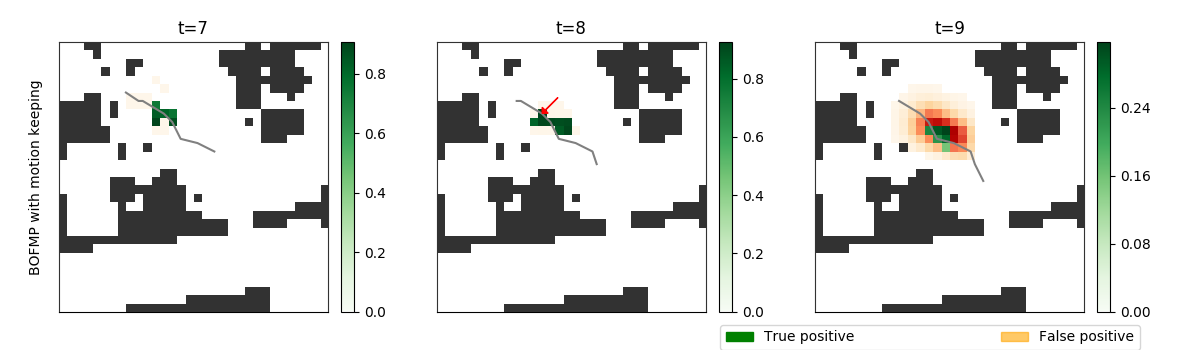
\includegraphics[width=\textwidth]{figures/moving_average_tracking.png}
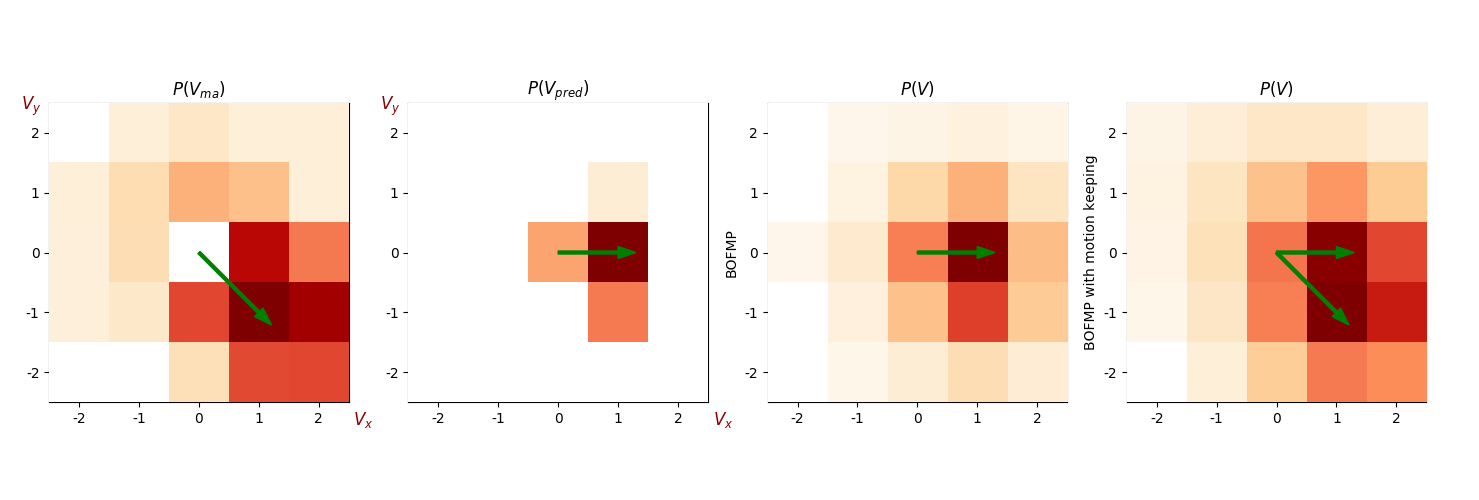
\includegraphics[width=\textwidth]{figures/moving_average_tracking_velocities_1.png}
\caption{\textbf{Up}: Three tracking steps of BOFMP with motion keeping. A person is walking from upper left towards lower right. The measurement is lost at $t=9$. \textbf{Down}: Velocities of the cell pointed by the red arrow at $t=8$. On each plot, the most possible direction is shown by the green arrows. Based on measurements from $t=7$ and $t=8$, the predicted velocity $P\{V_{pred}\}$ shows it is more likely the occupancy will propagates towards right for the next time step. However, past motion trend, which is represented by $P\{V_{ma}\}$, shows it is more likely to move to lower right. As a consequnce, BOFMP with motion keeping shows there are possibilities going both right and lower right, which is more realistic in this tracking example.}
\label{fig:keep_motion_idea}
\end{figure}


We randonly sample 100 sets of parameters for each scenario, evaluate them on validation set, and select the best set of parameters based on the mean of average precisions for the future prediction stage ($t=9:16$). The best parameters are shown in Table \ref{table:best_param_real}.

\begin{table}[H]
\footnotesize
\centering  
\begin{tabularx}{\textwidth}{c|c|c|c|c|c|c|c|c|c}
    \hline
    & $ e $ & $ \delta^2 $ & $ \Omega $ & \sml{blurExt} & \sml{blurVar} & $w$ & \sml{initMF} & \sml{keepMF}  & \footnotesize{mean a.p.}\\ \hline \hline
    BOFUM & 5 & 0.677 & 0.152  & - & - & - & - & - & 0.302   \\ \hline
    BOFMP & 5 & 0.649 & 0.191  & - & - & - & - & - & 0.321  \\
    \scriptsize{BOFMP spatial blurring} & 5 & 0.636 & 0.100  & 5 & 1.093 & - & - & - & 0.327  \\
    \scriptsize{BOFMP motion keeping} & 7 & 0.744 & 0.026  & - & - & 4 & 0.563 & 0.707 & 0.381  \\
   \hline
\end{tabularx}
\label{table:best_param_real}
\caption{Best parameters for BOFUM and BOFMP on real data.}
\end{table}

\normalsize
Then we apply each filter with its best parameters on test data of 244 tracking cases. Figure \ref{fig:real_test_data} shows the average precision for each time step, and Table \ref{table:real_test_data} lists the average precision in future prediction stage and their mean. Compared with BOFUM, our methods have performance gain of $29\%$, $31\%$ and $43\%$ respectively.

\begin{table}[H]
\footnotesize
\centering  
\begin{tabularx}{.8\textwidth}{c|c|c}
    \hline
    & average precision for $t=9:16$ & mean \\ \hline \hline
    BOFUM & 0.670   0.512  0.384  0.314  0.252  0.205  0.167  0.148  & 0.331   \\ \hline
    BOFMP & 0.705  0.570   0.468  0.424  0.351  0.336  0.305  0.255 & 0.427  \\
    \scriptsize{BOFMP spatial blurring} & 0.694  0.564  0.480   0.439  0.371  0.349  0.311  0.264 &  0.434  \\
    \scriptsize{BOFMP motion keeping} &  0.762  0.675  0.561  0.496  0.405  0.353  0.305  0.238 & 0.474  \\
   \hline
  \end{tabularx}
\label{table:real_test_data}
\caption{Future predictions for BOFUM and BOFMP on real data.}
\end{table}
\normalsize

\begin{figure}[ht]
  \centering
   \captionsetup{width=\linewidth}
    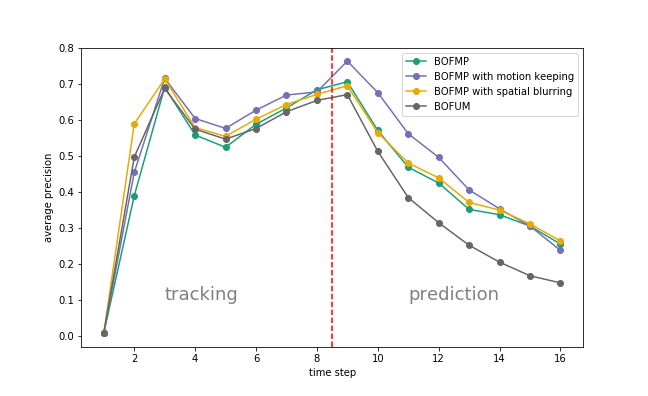
\includegraphics[width=.8\textwidth]{figures/test_on_real_data.png}
    \caption{Evaluation results on real test data. Like for simulated data, average precision starts with values close to zero, and increase rapidly over the next two time steps. From $t=3$ to $t=8$, average precisions keep rather stable at high values, which proves that filters predict very well for the next immediate step. In future prediction stage ($t=9:16$), average precisions decrease severely as time horizon increases, since the state of the world becomes more uncertain. However, our BOFMP and its variations are still better than BOFUM for every time step in this stage.}
    \label{fig:real_test_data}
\end{figure}

To conclude, we proposed a Bayesian occupancy filter that utilizes human motion pattern for tacking humans in indoor environments. The motion patterns are gained from a neural network which is trained on simulated human trajectories. Our proposed method outputforms BOFUM on both simulated and real tracking cases. One of the most important advantages of our method is that, although the motion pattern is derived from simulated data, it is applicable on real tracking scenarios.  













% Appendix (Anhänge), could have multiple chaper-files:
\appendix
\chapter{}
The appendix may contain some listings of source code that has been used for simulations, extensive proofs or any other things that are strongly related to the thesis but not of immediate interest to the reader. 

% Abbreviations (Abkürzungsverzeichnis):
\chapter{Notation und Abkürzungen}
This chapter contains tables where all abbreviations and other notations like mathematical
placeholders used in the thesis are listed.
\begin{table}[h]
\begin{tabular}{ll}
AP & Access Point\\
CQI & Channel Quality Indicator\\
DCI & Downlink Control Information\\
D-SR & Dedicated Scheduling Request\\
D2D & device to device\\
eNodeB & evolved Node B or E-UTRAN Node B\\
FDD & Frequency Division Duplexing\\
H-ARQ & Hybrid-Automatic Repeat Request\\
IoT & Internet of Things\\
LTE & Long Term Evolution\\
MCS & Modulation and Coding Scheme\\
OFDM & Orthogonal Frequency Division Multiplexing\\
PDCCH & Physical Downlink Control Channel\\
PDSCH & Physical Downlink Shared Channel\\
PRB & Physical Resource Block\\
PUCCH & Physical Uplink Control Channel\\
PUSCH & Physical Uplink Shared Channel\\
RACH & Random Access Channel\\
SC-FDMA & Single Carrier Frequency Division Multiple Access\\
SR & Scheduling Request\\
SRS & Sounding Reference Signal\\
TDD & Time Division Duplexing\\
UE & User Equipment\\
\end{tabular}
\end{table}




% References (Literaturverzeichnis):
% a) Style (with numbers: use unsrt):
\bibliographystyle{apalike}
% b) The File:
\bibliography{Bibliography}


%%%%%%%%%%%%%%%%%%%%%%%%%%%%%%%%%%%%%%%%%%%%%%%%%%%%%%%%%%%%


%%%%%%%%%%%%%%%%%%%%%%%%%%%%%%%%%%%%%%%%%%%%%%%%%%%%%%%%%%%%


%%%%%%%%%%%%%%%%%%%%%%%%%%%%%%%%%%%%%%%%%%%%%%%%%%%%%%%%%%%%
\end{document}
